 %美赛模板:正文部分

\documentclass[12pt]{article}  % 官方要求字号不小于 12 号,此处选择 12 号字体
% \linespread{1.1}
% \bibliographystyle{plain}
% 本模板不需要填写年份,以当前电脑时间自动生成
% 请在以下的方括号中填写队伍控制号
\usepackage[2501426]{easymcm}  % 载入 EasyMCM 模板文件
\problem{B}  % 请在此处填写题号
% \usepackage{mathptmx}  % 这是 Times 字体,中规中矩 
\usepackage{palatino}  % mathpazo 这palatino是 COMAP 官方杂志采用的更好看的 Palatino 字体,可替代以上的 mathptmx 宏包
\usepackage{pdfpages}
\usepackage{longtable}
\usepackage{tabu}
\usepackage{lastpage}
\usepackage{threeparttable}
\usepackage{xcolor}
\usepackage{listings}

\definecolor{mygreen}{rgb}{0,0.6,0}
\definecolor{mygray}{rgb}{0.5,0.5,0.5}
\definecolor{mymauve}{rgb}{0.58,0,0.82}

\lstset{
	language=Python,
	basicstyle=\ttfamily,
	numbers=left,
	numberstyle=\tiny\color{mygray},
	breaklines=true,
	frame=single,
	showstringspaces=false,
	keywordstyle=\color{blue},
	morekeywords={True, False, None}, % 添加额外的关键字
	commentstyle=\color{mygreen},
	stringstyle=\color{mymauve},
}

\usepackage{paralist}
\graphicspath{{img/}}          % 此处{img/}为相对路径,注意加上“/”
 \let\itemize\compactitem
 \let\enditemize\endcompactitem

\newcommand{\upcite}[1]{\textsuperscript{\textsuperscript{\cite{#1}}}}
\title{An investment theory model based on linear programming}  % 标题

% 如需要修改题头(默认为 MCM/ICM),请使用以下命令(此处修改为 MCM)
%\renewcommand{\contest}{MCM}

 %文档开始
\begin{document}

% 此处填写摘要内容
\begin{abstract}
% 下面是设置缩进
\setlength{\parindent}{2em}
	
	% (Need to be reviewed)
	Emerging industries are booming and mobilizing rapid economic growth, and this paper provides a discussion of the problems posed by the interaction of the industries, modeling how to promote the industries as well as increase employment to achieve economic sustainability.

	To address question 1, the annual growth rates of the nine industries were first calculated. The correlation and causality of each group of industries is quantified by grouping the industries in pairs and applying Pearson's correlation coefficient and Granger causality test. Then, based on the correlation coefficients of each group, the impact between them and on economic development is evaluated.

	To address question 2, the investment and GDP of each industry were used separately using linear regression, the goodness of fit was calculated, and the accuracy of the fit was tested using the coefficient of determination ${R^2}$ to derive a theoretical model of investment and GDP for each industry.

	For Problem 3, the particle swarm algorithm is used to construct an objective function to maximize GDP, set up constraints to see that the industries that maximize profits are industry, wholesale and retail trade, and other industries, and solve the equation to arrive at an optimal investment ratio of $30.9\%:52.6\%:16.5\%$.

	For problem 4, the elasticity values were calculated by replacing the original values with the elasticity values. Normalizing it and further calculating it to get the composite elasticity value and allocating the investment ratio of $39.21\%:30.41\%:30.39\%$ according to the size of the elasticity value to the other sectors, finance and transport, storage and postal services will maximize the value of production.

	For problem 5, a multi-objective planning model is constructed to maximize the employment rate and GDP, using hierarchical analysis to give weights to the variables to establish the objective function through the particle swarm algorithm to obtain the optimal solution for the industry, other industries and wholesale and retail trade investment ratio of $32.6\%:18.6\%:9.8\%$.

	
	% Here is the abstract of your paper.
	
	% Firstly, that is ...
	
	% Secondly, that is ...
	
	% Finally, that is ...
	
	% 美赛论文中无需注明关键字。若您一定要使用,
	% 请将以下两行的注释号 '%' 去除,以使其生效
	\vspace{5pt}
	\textbf{Keywords}: Granger Causality Test; Tarticle Swarm Algorithm; Multi-Objective Optimization; Hierarchical Analysis;
	
\end{abstract}

\maketitle  % 生成 Summary Sheet

\tableofcontents  % 生成目录


% 正文开始
% Chapter 1: Introduction
\section{Introduction}

\subsection{Problem Background} %背景介绍

	Guided by Xi Jinping's thought of socialism with Chinese characteristics in the new era, it comprehensively implements the spirit of the Third Plenary Session of the 20th CPC Central Committee and promotes the development of the national economy. China's industrial structure has also undergone significant changes, and emerging industries have flourished. Compared with the traditional manufacturing industry, emerging industries have provided new impetus for China's economic growth, and have had a profound impact on economic development as well as the economic landscape. At present, the interrelationships between domestic industries have various impacts, and this paper examines this issue.


%\begin{figure}[htbp]  %h此处,t页顶,b页底,p独立一页,浮动体出现的位置
%\centering  %图表居中
%\includegraphics[width=.7\textwidth]{Fire_Situation.png} %图片的名称或者路径之中有空格会出问题 
%\caption{Fire Situation in Australia (Feb 2020 - Feb 2021)} % 图片标题 
%\label{fig:Fire Situation} % 图片标签,可以不写
%\end{figure}



\subsection{Restatement of the Problem} %问题重述
%文字内容
	The interrelationships between domestic industries are intricate and complex, and this paper will comprehensively consider the complexity and industrial interconnectedness of these industries with the aim of achieving balanced and sustainable economic growth, enhancing employment, and focusing on the following problems:


%列表
\begin{itemize} %拟解决的问题
\setlength{\parsep}{0ex} %段落间距
\setlength{\topsep}{2ex} %列表到上下文的垂直距离
\setlength{\itemsep}{1ex} %条目间距
\item Question 1: Collect data related to major domestic industries and analyze and discuss the interrelationships within China's major industries and their impact on economic development.
\item Question 2: Design one or more theoretical models of investment, study the relationship between investment and the gross domestic product of various industries, and evaluate the models.
\item Question 3: Analyze the percentage allocation of investments in all or only three types of industries to achieve the highest GDP using a total investment fund of 1 trillion units.

\item Question 4: Analyze the proportion of investment allocated to all or just three types of industries that use 1 trillion units to effectively stimulate employment.
\item Question 5: Optimize investment plans to ensure a steady increase in employment while increasing GDP.
\end{itemize}

%\subsection{Literature Review} %文献综述
%文字内内容

%%列表
%\begin{itemize}
%\setlength{\parsep}{0ex} %段落间距
%\setlength{\topsep}{2ex} %列表到上下文的垂直距离
%\setlength{\itemsep}{1ex} %条目间距  这三句如果删除就是各条贴在一起
%\item 
%
%\item
% 
%\item 
%
%\item 
%
%\end{itemize}


\subsection{Our Work} %工作分配
The problem requires us to fight fires by optimizing the locations of two type of drones. In order to avoid complicated description, intuitively reflect our work process, the flow chart is shown in Figure 1:


\begin{figure}[H]  %h此处,t页顶,b页底,p独立一页,浮动体出现的位置
\centering  %图表居中
\label{ourwork}
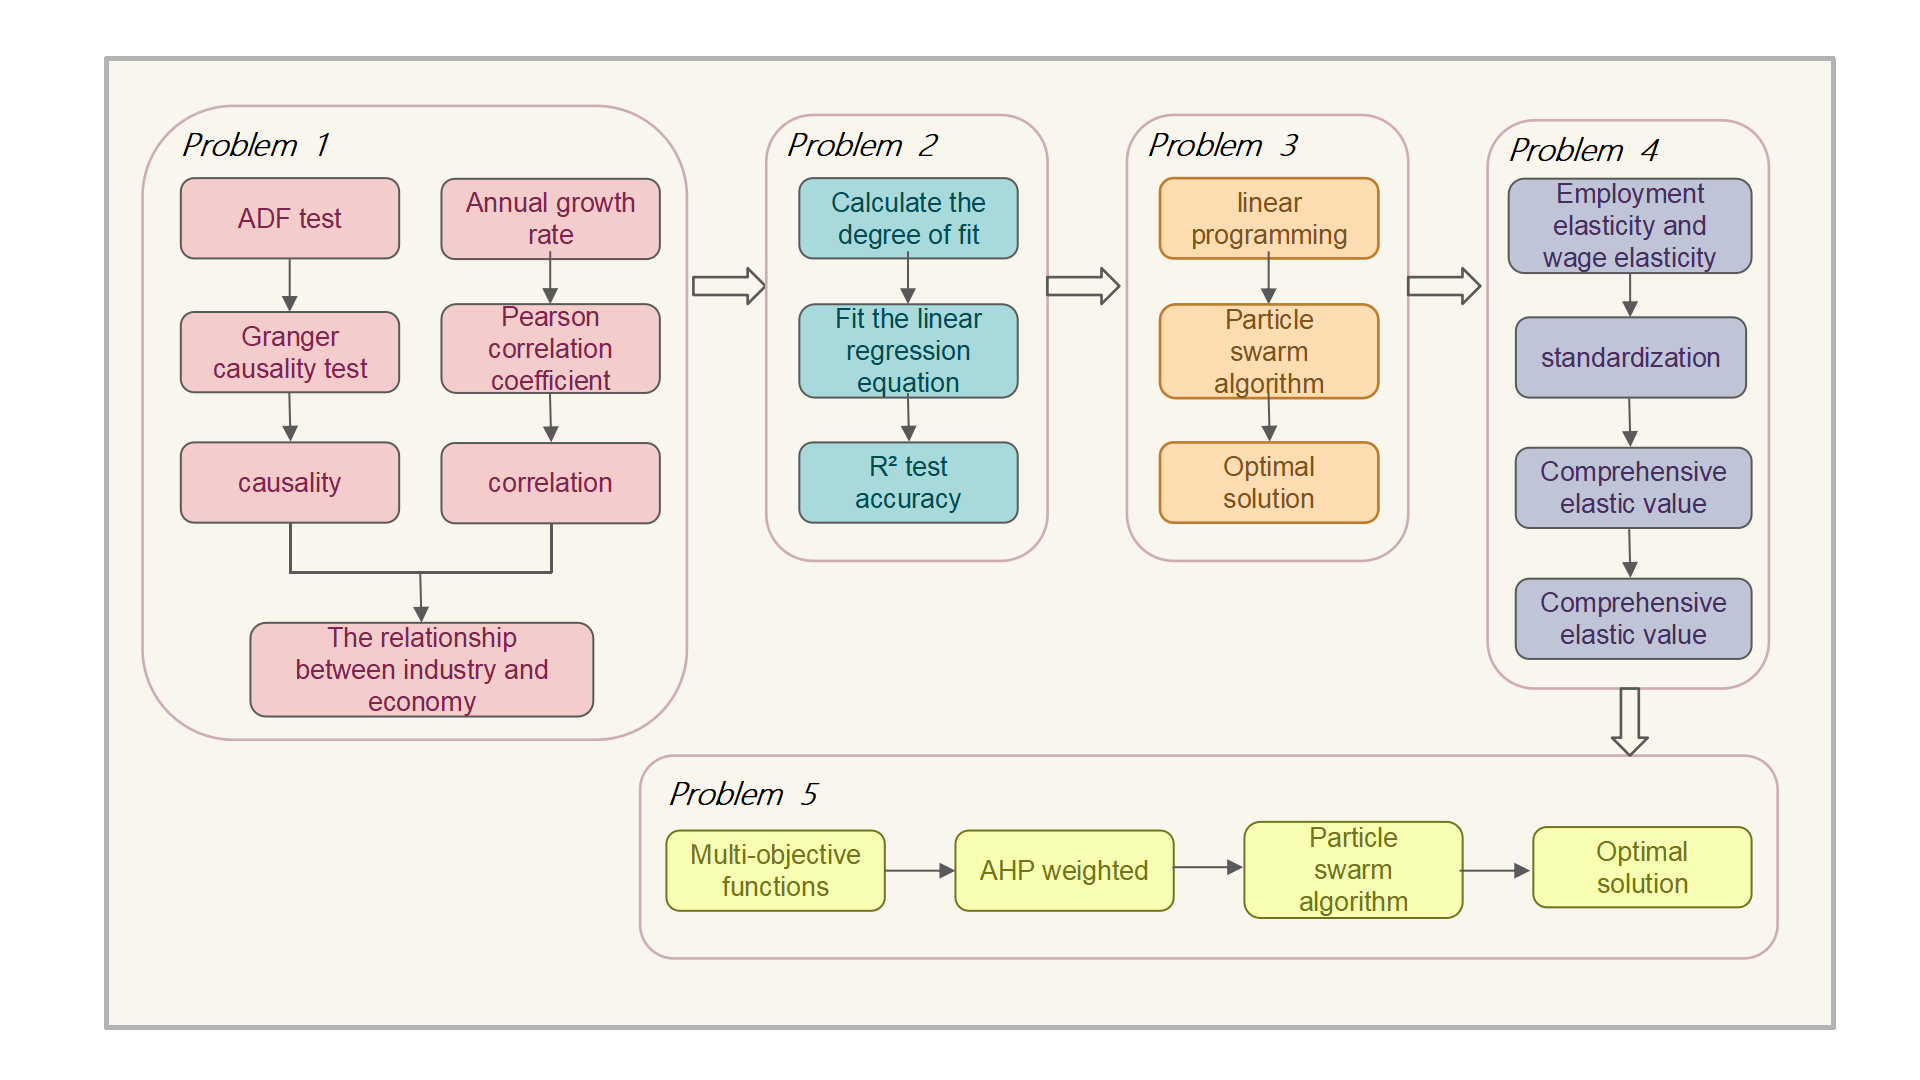
\includegraphics[width=.9\textwidth]{img/our_work.png} %图片的名称或者路径之中有空格会出问题 
\caption{Ourwork} % 图片标题 
\end{figure}
\vspace{-0.8cm}

\section{Analysis of Problems} %问题分析
\subsection{Analysis of problem 1} % 问题分析1
	The major industries in China include agriculture, forestry, animal husbandry and fishery, industry, construction, wholesale and retail trade, transportation, storage and postal service, accommodation and food service, finance, real estate, and other industries. Gross product and GDP of each industry in recent years were collected from the National Bureau of Statistics to analyze the year-on-year growth rate of the industry. By calculating the Pearson's correlation coefficient between each two industries, explore the interactions between industries and their role in the economy.
	
\subsection{Analysis of problem 2} % 问题分析2
	An investment theory model is a theoretical framework used to analyze and predict investment behavior and its impact on the economy. Therefore, we utilize a linear regression model to derive the fitted parameters for each industry for each year using known data, which forms the core of the investment theory model. Finally, the fitted parameters are evaluated to ensure the accuracy and reliability of the model.

\subsection{Analysis of problem 3} % 问题分析3
	To maximize the benefits, it is necessary to predict the changes in the gross product of each industry and analyze the changes in the total economic value of the industry. Therefore, the future gross product of each industry can be predicted through the fitting function derived from problem two. According to the proportion of each industry to divide the amount of investment, in the proportion of the size of the first three industries as the three industries limited to investment, and finally through the proportion of the division of 1 trillion dollars of investment.
	
\subsection{Analysis of problem 4} % 问题分析4
	To improve the employment rate as well as the quality of employment, two factors should be considered: the employed population and the wages of jobs. Firstly, the data is cleaned in order to ensure the integrity and consistency of the data. Secondly, we calculate the growth rate of employment population and wages in each industry, through which we calculate the employment elasticity and wage elasticity, take the average of the elasticity values, calculate the comprehensive elasticity value, and then get the investment allocation of each industry, and choose the three industries with the highest comprehensive elasticity for investment.

\subsection{Analysis of problem 5} % 问题分析5
	To improve the employment rate as well as the quality of employment, two factors should be considered: the employed population and the wages of jobs. Firstly, the data is cleaned in order to ensure the integrity and consistency of the data. Secondly, we calculate the growth rate of employment population and wages in each industry, through which we calculate the employment elasticity and wage elasticity, take the average of the elasticity values, calculate the comprehensive elasticity value, and then get the investment allocation of each industry, and choose the three industries with the highest comprehensive elasticity for investment.

\section{Model Assumptions} % 模型假设
	This paper makes the following assumptions to address the above questions:
\begin{enumerate}[\bfseries \textit{Assumption} 1:]

%假设1
	\item \textbf{Only the movement of the entire investment is considered, without specifically distinguishing between specific forms of cash flows such as own funds and borrowed funds.}\\
%解释1
%	\textbf{\textit{Explanation:}}
	
	
		\item \textbf{Errors arise only from science and technology, policy, labor, etc. and are not related to force majeure factors.}\\
	
%		\textbf{\textit{Explanation:}}
		
		
%			\item \textbf{}\\
			
%			\textbf{\textit{Explanation:}}
			
			
%				\item \textbf{}\\
				
%				\textbf{\textit{Explanation:}}
\end{enumerate}


\section{Notations}%符号说明
Some important mathematical notations used in this paper are listed in Table 1. 
\begin{table}[htbp]
	\centering
	\caption{Model assumptions.}
	\label{tab:notations}
	\begin{tabular}{ll}
		\toprule
		\textbf{Notation} & \textbf{Hidden Meaning} \\
		\midrule
		$S_1$ & Gross Domestic Product (GDP) \\
		$S_2$ & Agriculture, forestry, animal husbandry and fisheries \\
		$S_3$ & Industries \\
		$S_4$ & Building industry \\
		$S_5$ & Wholesale and retail trade \\
		$S_6$ & Transportation, storage and postal services \\
		$S_7$ & Accommodation and catering \\
		$S_8$ & Financial sector \\
		$S_9$ & Real estate industry \\
		$S_{10}$ & Other industries \\
		$r$ & Pearson correlation coefficient \\
		$R^2$ & Coefficient of determination (CoD) \\
		$\alpha_i$ & Return on investment (ROI) \\
		\bottomrule
	\end{tabular}
\end{table}

\vspace{-1cm}%在\end{table}下加一行\vspace{-1cm} 其中-1的作用是缩短与下方文字距离的 切记!必须是负数

\section{Model Preparation} %建模准备
\subsection{Modeling based on Pearson's correlation coefficient for solving} %数据概览
%文字内容
	The Granger causality test\cite{1} is utilized to study the interactions between major industries in China, and the Pearson correlation number\cite{2} is used to study the relationship between industries, and the two methods are combined to study the impact on economic development.

\subsubsection{Preparation Based on the Pearson Correlation Coefficient Model} %数据采集
	Before the model is built, ADF test should be carried out on the data of GDP and Gross Domestic Product (GDP) of each industry in recent years to determine whether the time series is smooth or not.
	
\subsubsection{Establishment Based on the Pearson Correlation Coefficient Model} %数据采集

	The data shows that, to date, the gross output of various industries has been on an upward trend. From a statistical perspective, the Granger causality test can be applied to the gross outputs of various industries over the past 20 years ($S_{2}$, $S_{3}$, $S_{4}$, $S_{5}$, $S_{6}$, $S_{7}$, $S_{8}$, $S_{9}$ and $S_{10}$) and 10 indicators including $S_{1}$, to examine whether causal relationships exist between the indicators. The specific steps for the Granger causality test are illustrated in the following figure:
	% 图
	
	The following regression model was developed based on the lag order:
	\begin{equation}
	{C_t} = \alpha  + {\beta _1}{C_{t - 1}} + {\beta _2}{C_{t - 2}} + {\gamma _1}{D_{t - 1}} + {\gamma _2}{D_{2 - 1}}
	\end{equation}

	where $C_t$ is the consumption expenditure of an industry in the first $t$ period, $C_{t-1}$ and $C_{t-2}$ are the lagged terms of the consumption expenditure of the industry, $D_{t-1}$ and $D_{t-2}$ are the lagged terms of another industry, $\alpha$ is a constant term, and $\beta_1$, $\beta_2$, ${\gamma_1}$ and ${\gamma_2}$ are the parameters to be estimated.
	
	In testing whether an industry is a Granger cause of consumer spending, the original hypothesis($H_0$) is that the industry is not a Granger cause of consumer spending. The alternative hypothesis($H_1$) is that the industry is a Granger cause of consumption expenditure. The same is true when testing consumption expenditure.
	
	The original hypothesis is usually tested using the $F$ test, where the expression for the statistic $F$ is:
	\begin{equation}
	F = \frac{{(RS{S_r} - RS{S_u})/q}}{{RS{S_u}/(n - k)}}
	\end{equation}

	Where $RS{S_r}$ is the residual sum of squares for the restricted model, $RSS_u$ is the residual sum of squares for the unrestricted model, $q$ is the number of parameters restricted, $n$ is the sample size, and $k$ is the number of parameters for the unrestricted model.
	
	Comparing the $F$ statistic from the above calculations with the critical value of the $F$ distribution gives an indication of whether one industry is the Granger cause of another.
	
	At the same time, GDP is analyzed by treating it as a more visual growth rate. First, any two industries are divided into a group, using $X$ to indicate one industry in a group and $Y$ to indicate another industry in a group. The Pearson's correlation coefficient is calculated with the change of growth rate of each industry in recent years, so as to present the relationship between each group of industries.
	
	Calculate the year-to-year growth rate for the raw data:
	\begin{equation}
		a = (\frac{{{b_j} - {b_{j - 1}}}}{{{b_{j - 1}}}}) \cdot 100\%
	\end{equation}

	where denotes the annual growth rate of the total output of the industry, ${b_j}$ ($j = 1, 2, \cdots, n $) denotes the GDP of an industry in the year $b$, and $b_{j-1}$ ($j = 1, 2, \cdots, n $) denotes the GDP of another industry in the year $j-1$.
	
	Pearson correlation coefficient was calculated based on the growth rate:
	\begin{equation}
	r = \frac{{\sum\limits_{i = 1}^n {({X_i} - \overline X )({Y_i} - \overline Y )} }}{{\sqrt {{{\sum\limits_{i = 1}^n {({X_i} - \overline X )} }^2}} \sqrt {{{\sum\limits_{i = 1}^n {({Y_i} - \overline Y )} }^2}} }} , i = 1, 2, \cdots, n 
	\end{equation}

	where $n$ denotes the total number of years to be calculated, $i$  denotes the year, $X_i$ and $Y_i$ denote the growth rate of GDP in the first $i$ year respectively. $\overline{X}$ and $\overline{Y}$ denote the average of the growth rates in the sample totals, respectively. 
	
	Calculate each group of data one by one to get the correlation coefficient between each two industries and analyze the correlation. The larger the value of  $\left| {\rm{r}} \right|$, the stronger the correlation; conversely, the smaller the value of $\left| {\rm{r}} \right|$, the weaker the correlation.
	
%\begin{table}[htbp] % 三线表
%\begin{center}
%\caption{Data and Database Websites}
%\resizebox{\textwidth}{!}
%{\begin{tabular}{c c}
%\toprule[2pt]
%\multicolumn{1}{m{5cm}}{\centering \textbf{Database Names}}
%&\multicolumn{1}{m{10cm}}{\centering \textbf{Database Websites} }\\ %m后面是列宽
%\midrule
%Fire Alerts& https://www.globalforestwatch.org/map/ \\
%Altitude & https://search.earthdata.nasa.gov/search \\
%Latitude and Longitude & https://www.kaggle.com/carlosparadis/\\ 
%Google Scholar & https://scholar.google.com/ \\
%Maps& \copyright{} 2021 Mapbox \copyright{} OpenStreetMap\\
%\bottomrule[2pt]
%\end{tabular}}
%\end{center}
%\end{table}

\subsubsection{Solution Based on The Pearson Correlation Coefficient Model} %数据甄别
%文本内容 
From the analysis of the ADF test results, it can be seen that the gross domestic product and GDP of each industry are smooth time series.Granger causality test was conducted using SPSSPRO on 10 data of China's industries and GDP in the last 20 years to get the comparison of significance level of 90 groups of industries as shown in the figure below.

\begin{figure}[H]
	\centering
	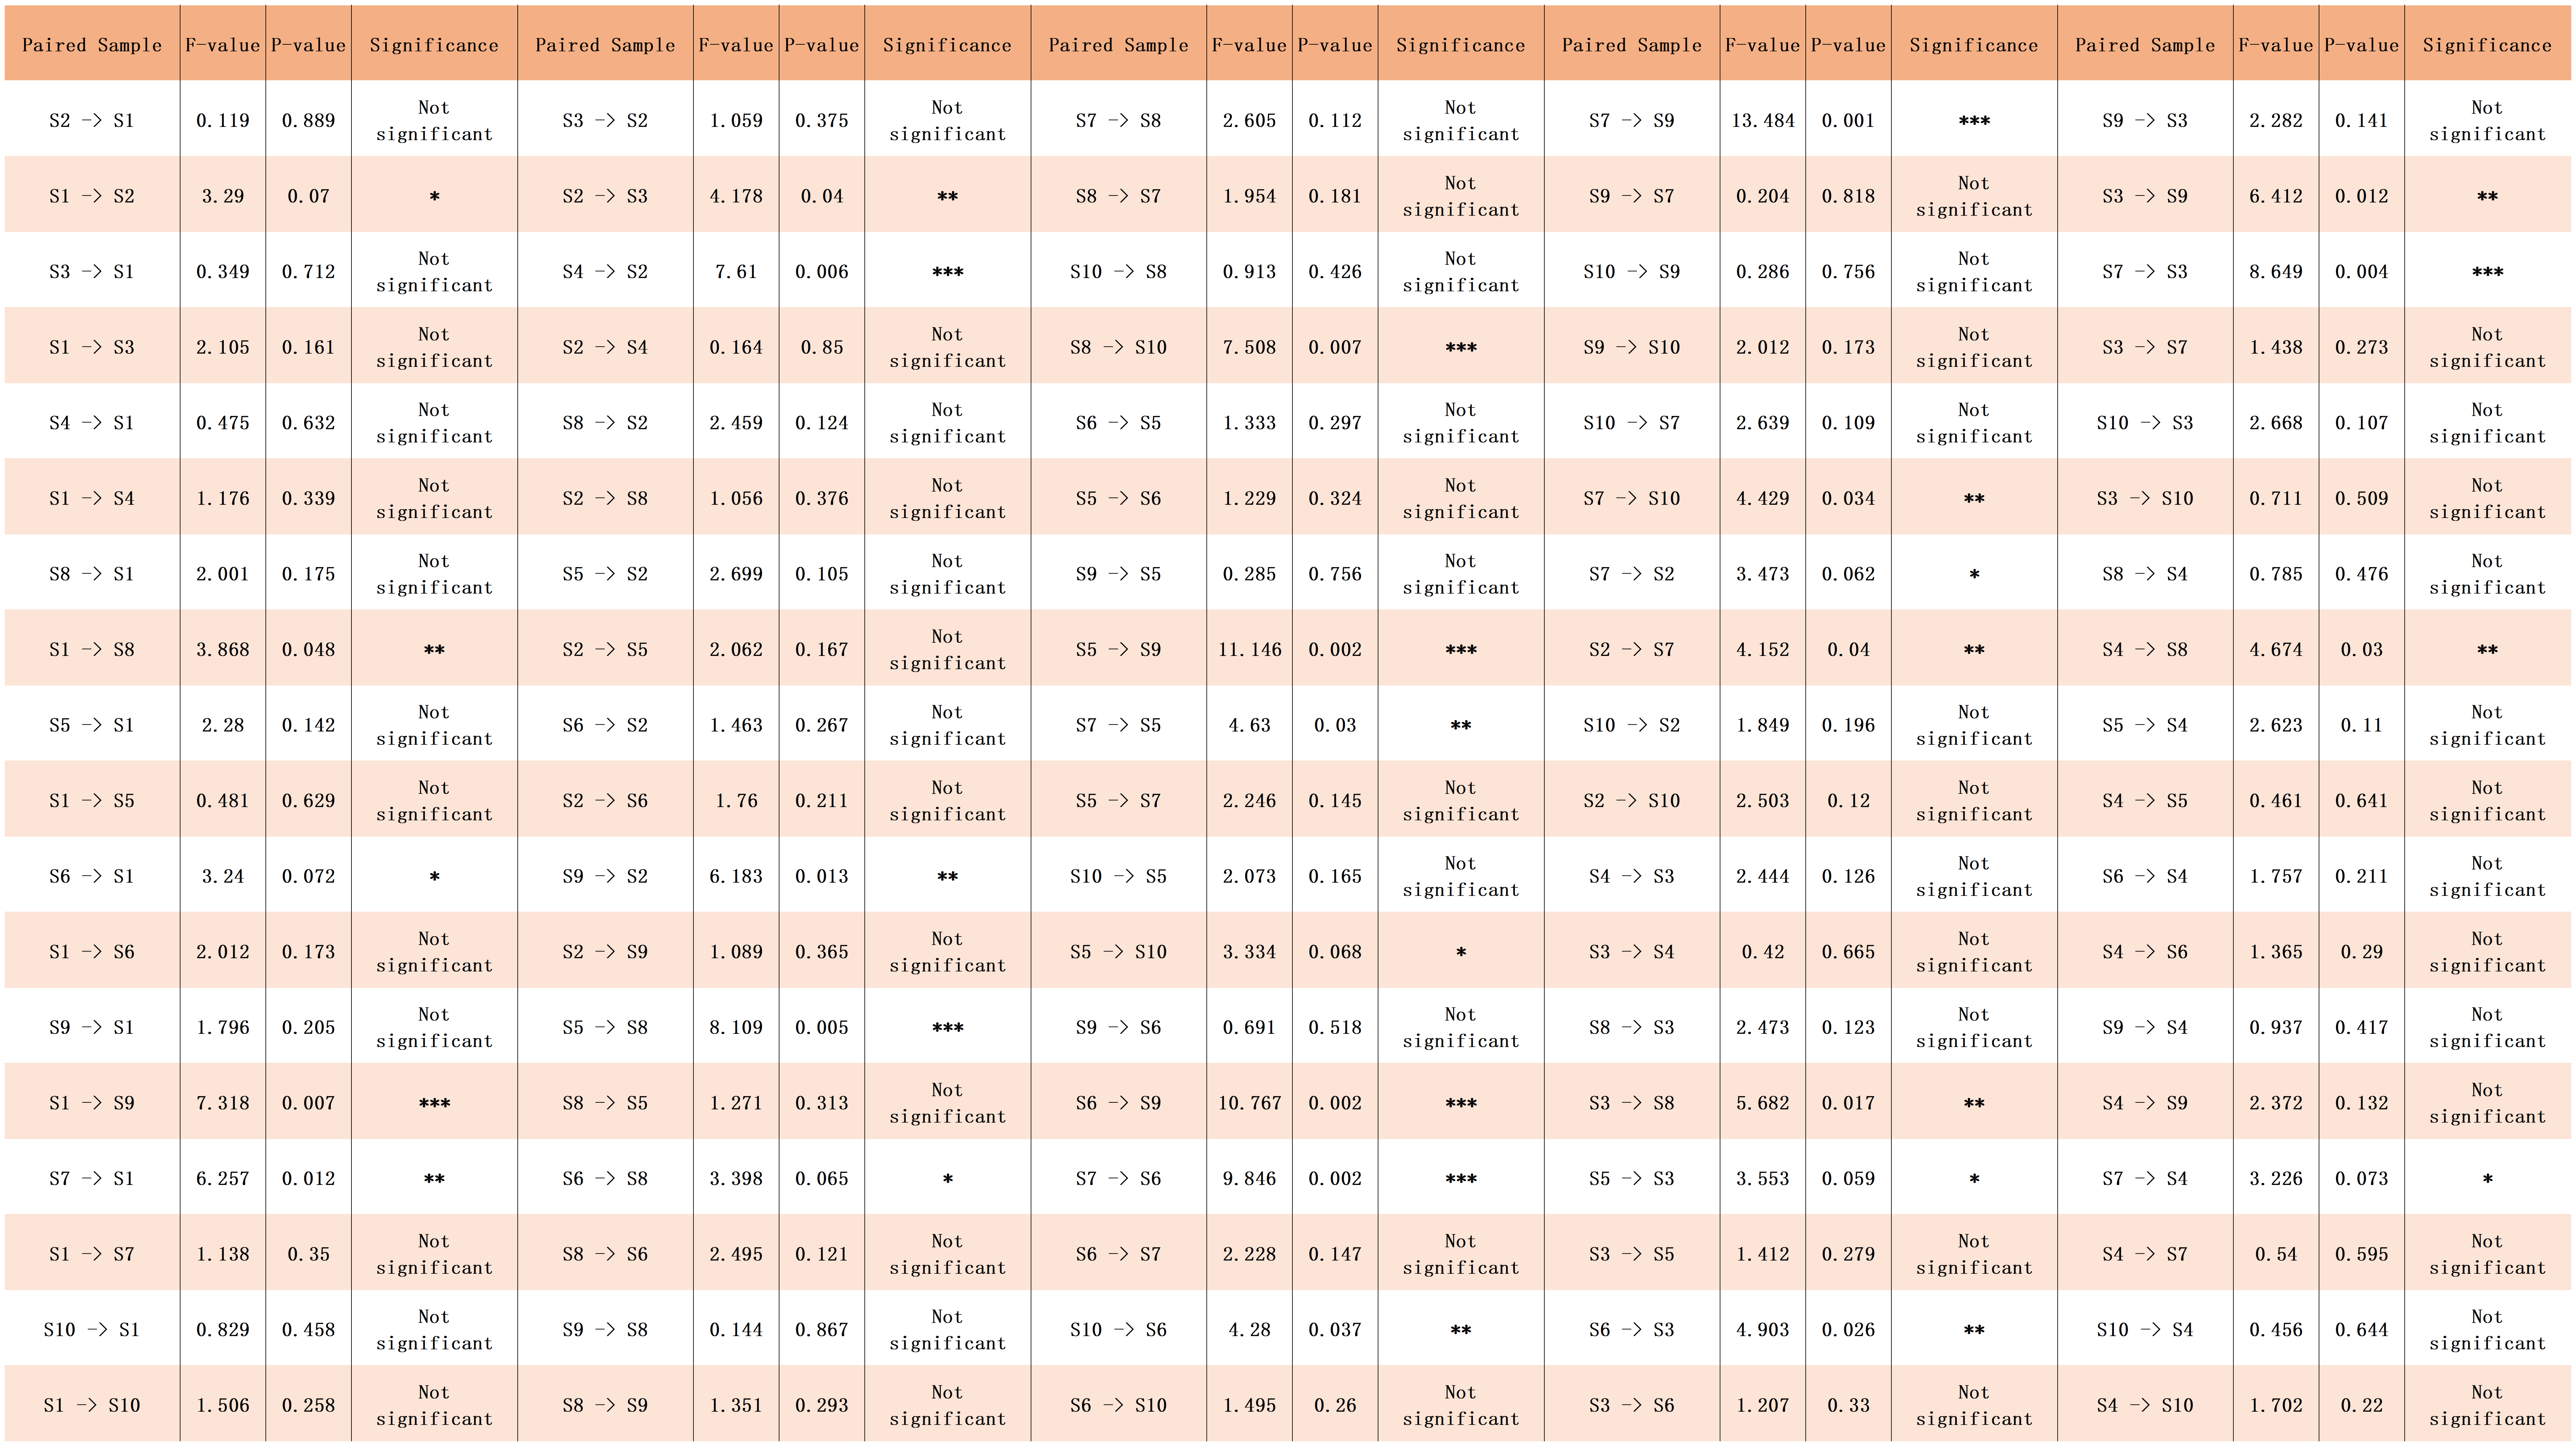
\includegraphics[width=1\textwidth]{img/q1_spsspro}
	\caption{Comparison of significance levels.}
	\label{figure1}
\end{figure}

	In the above table, ***, **, and * represent 1\%, 5\%, and 10\% significance levels, respectively.

	A significant $p < 0.05$ indicates the rejection of the original hypothesis (that one set of time series is not the cause of the other set of time series), i.e., the left-hand side variables can cause changes in the right-hand side variables with Granger causality, and vice versa, there is no Granger causality. In addition, the smaller the value of $p$, the more significant the difference between the observed data and the original hypothesis.
	
	In response to the results of the data in the above table, there is Granger causality between the following industries.
	
	\begin{figure}[H]
		\centering
		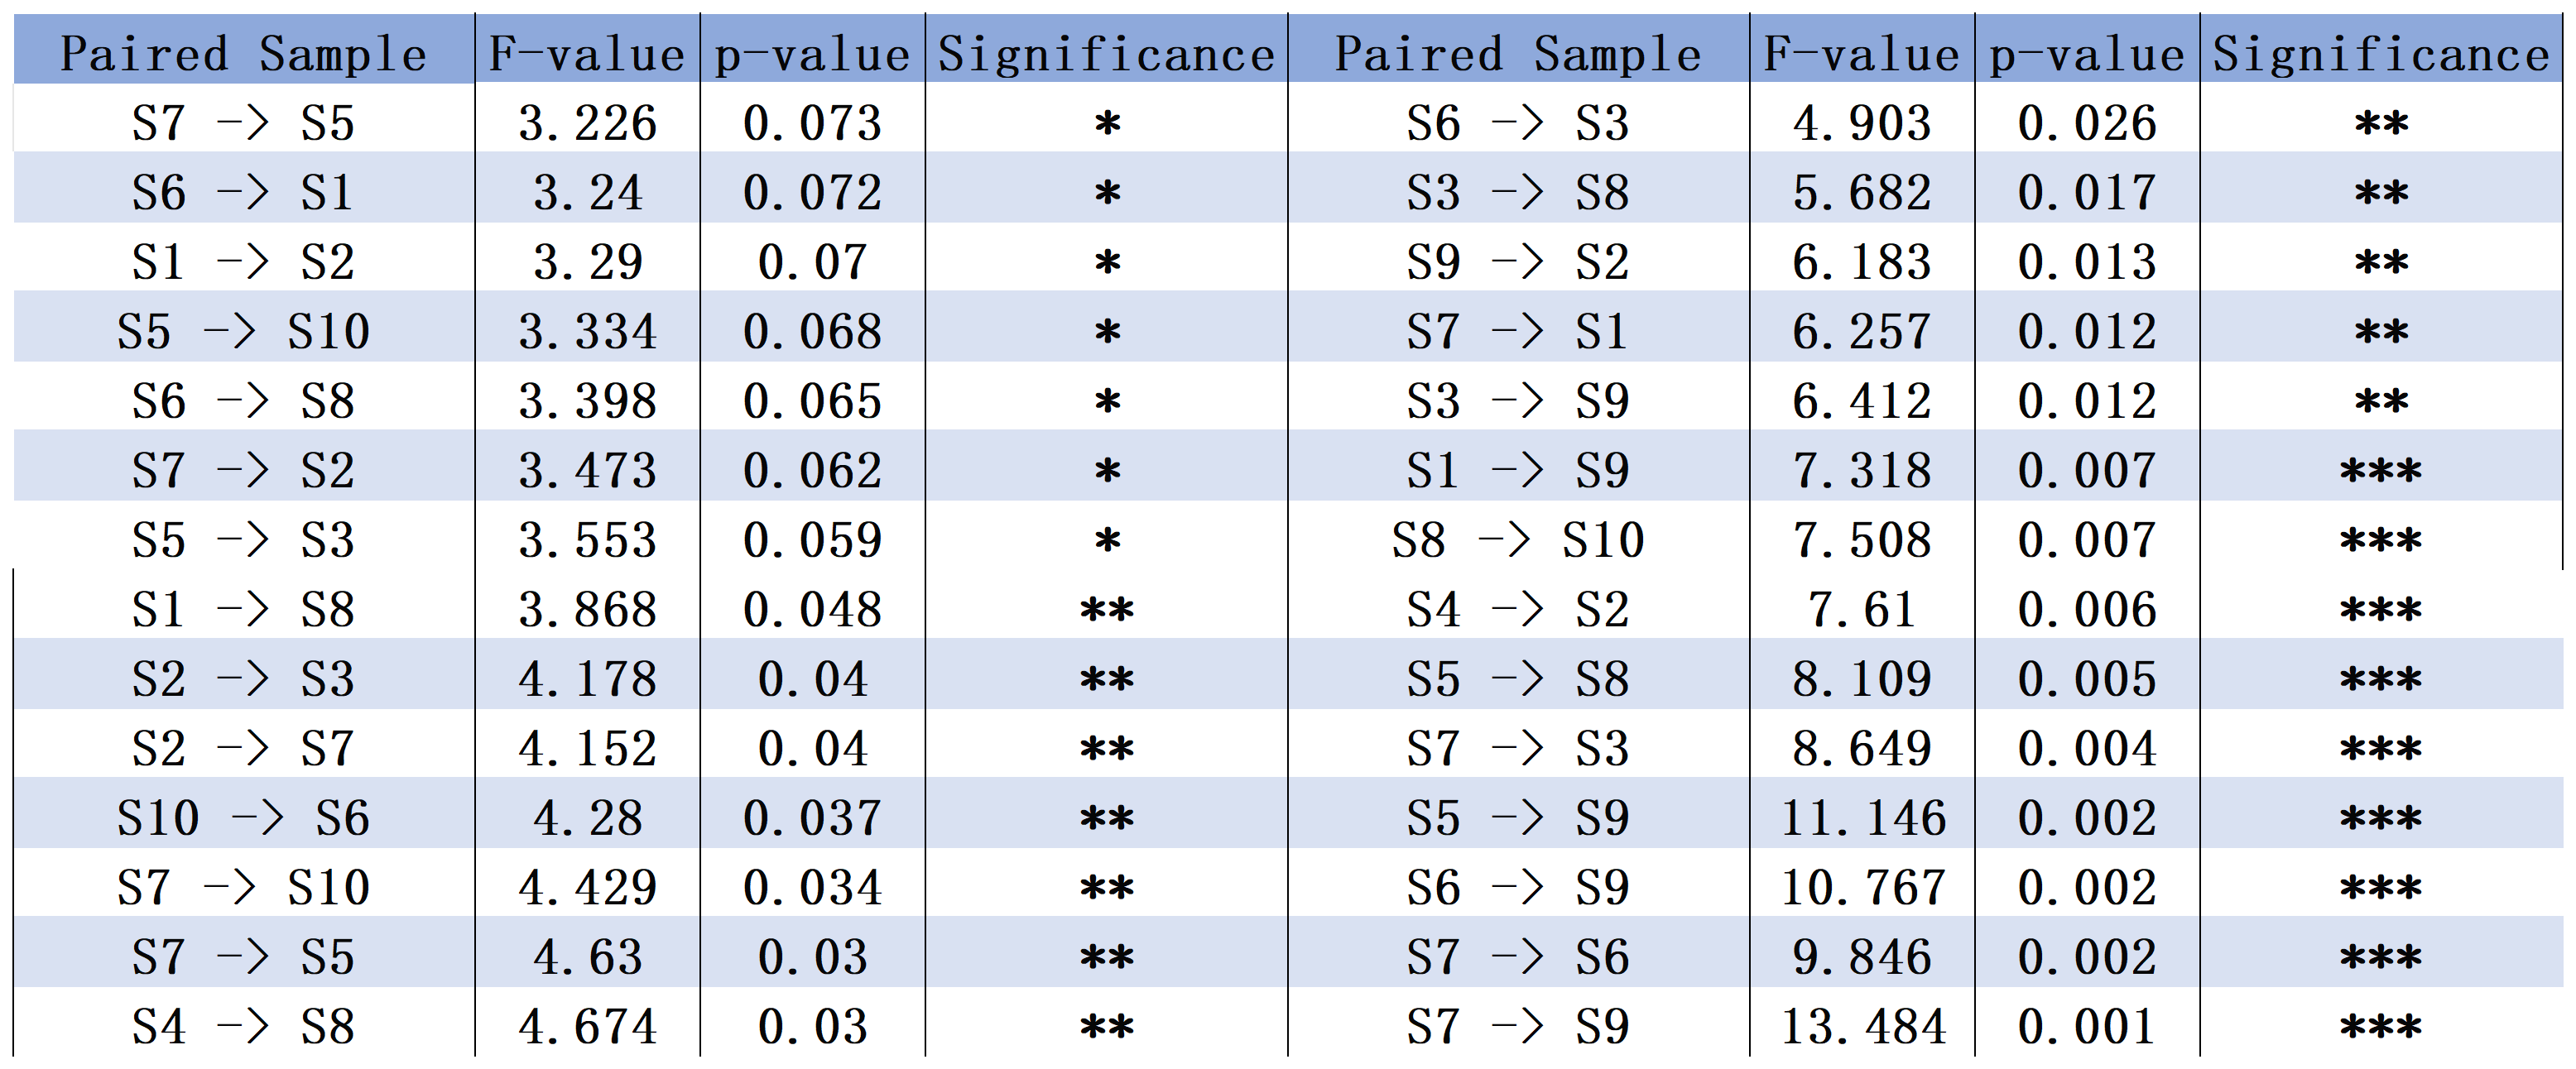
\includegraphics[width=1\textwidth]{img/q1_spsspro2}
		\caption{Granger causality.}
		\label{figure2}
	\end{figure}

	Among them, $S_7$ can directly affect $S_9$, $S_6$ and $S_3$, finance can directly affect other industries, construction can directly affect agriculture, forestry and fisheries, wholesale and retail trade can directly affect finance and real estate, and transportation, warehousing and postal services can directly affect real estate.
	
	At the same time, the economic growth rate of each group of different industries is calculated using matlab to get the change in growth rate of each group of data during 2004-2023 years.The following figure shows the line graph of the change in the growth rate of each industry over a period of 20 years.
	
	\begin{figure}[H]
		\centering
		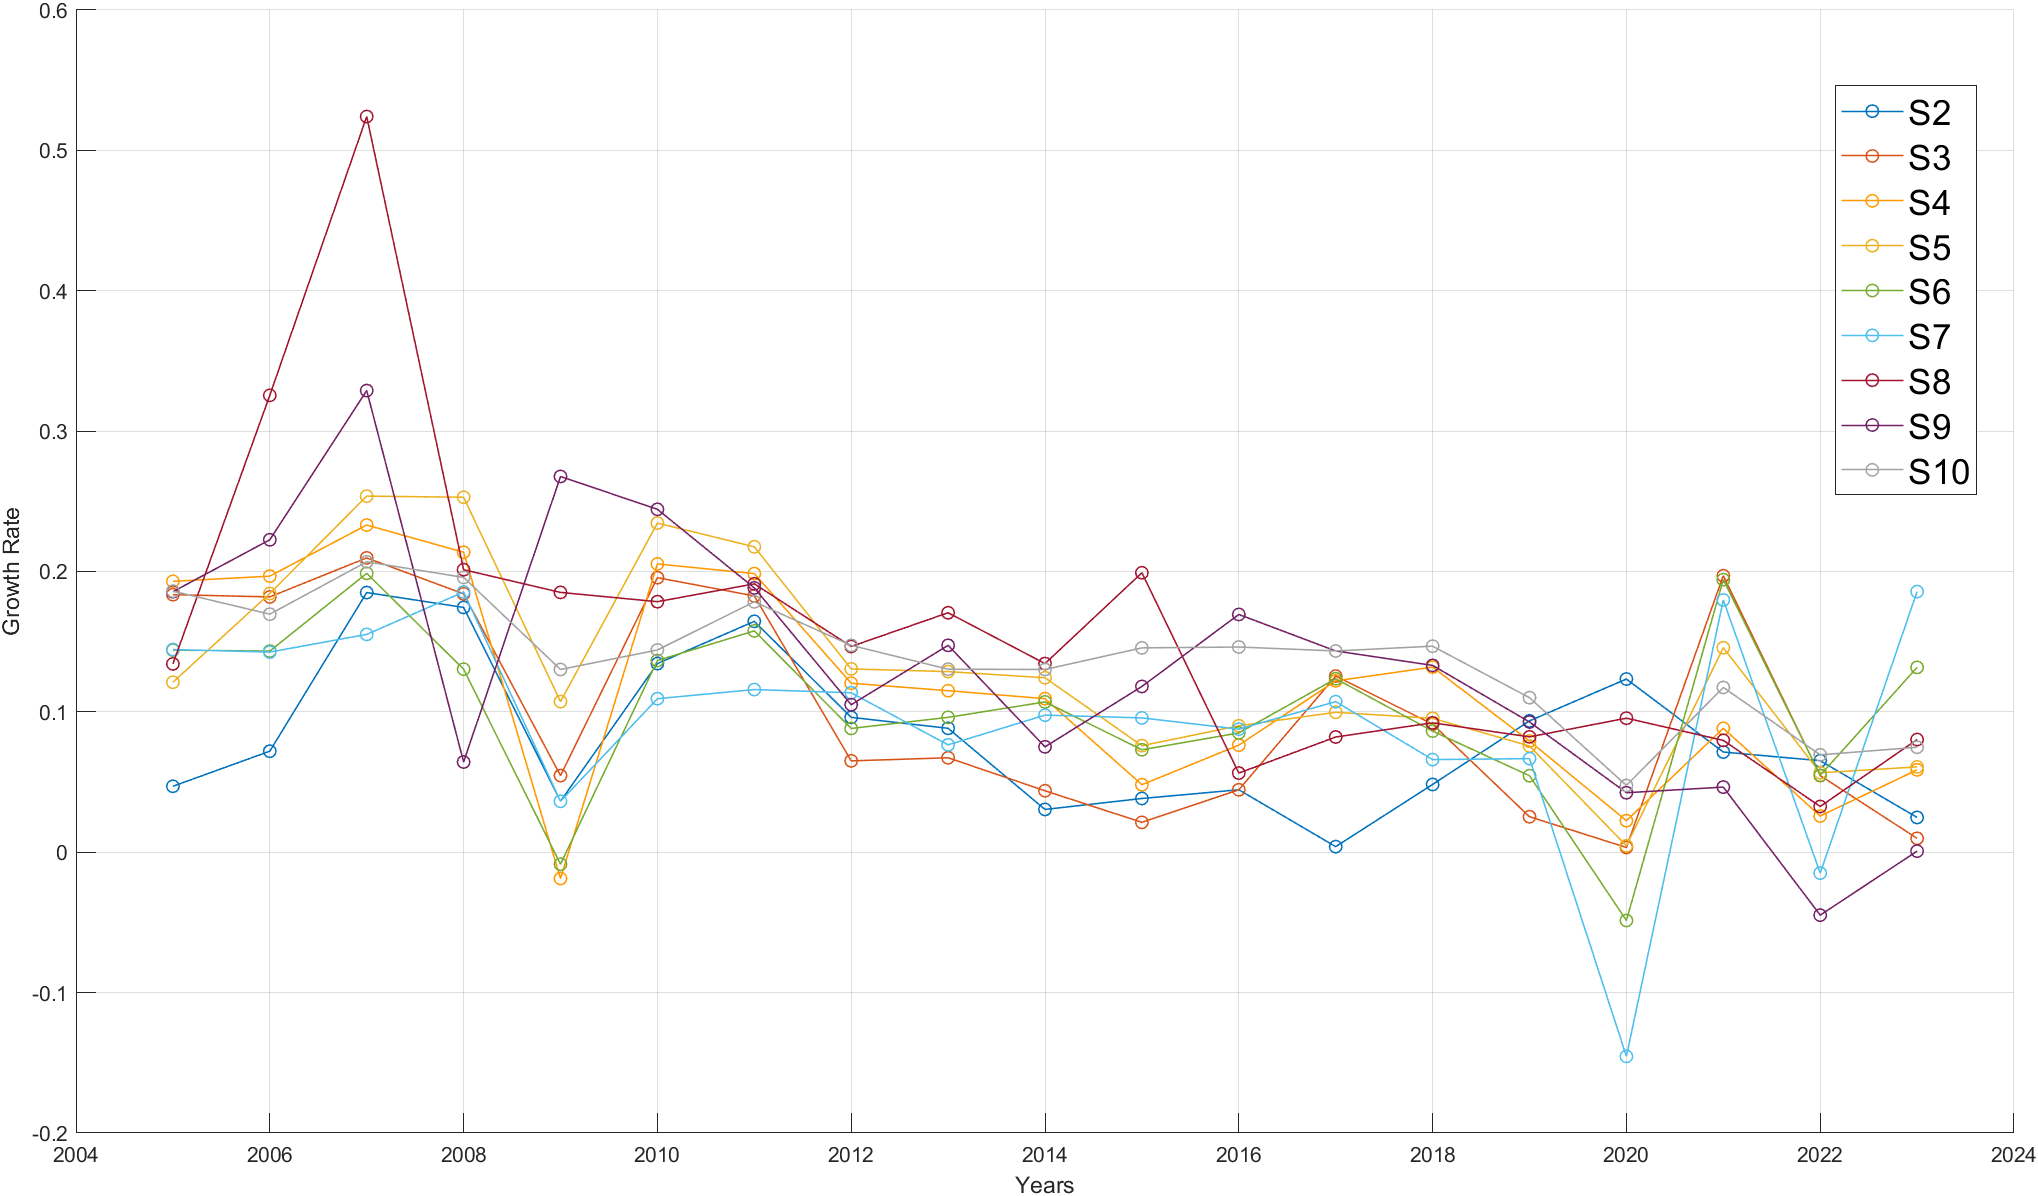
\includegraphics[width=0.9\textwidth]{img/q1_Line_20}
		\caption{Growth rate over 20 years.}
		\label{figure3}
	\end{figure}

	From the results of the above graph, it can be seen that in these 20 years, the vast majority of the industries had positive annual growth rates, i.e., the gross product of the industry showed an upward trend. However, in the year 2020, the impact of the New Crown Epidemic led to a downward trend in the gross product of most of the industries. Among them, the accommodation and food service industry showed a negative growth rate due to the tourism industry being more affected.
	
	The data from the above graph was brought into the Pearson correlation coefficient formula to calculate the correlation between each of the two industries to obtain the following heat map.
	
	\begin{figure}[H]
		\centering
    		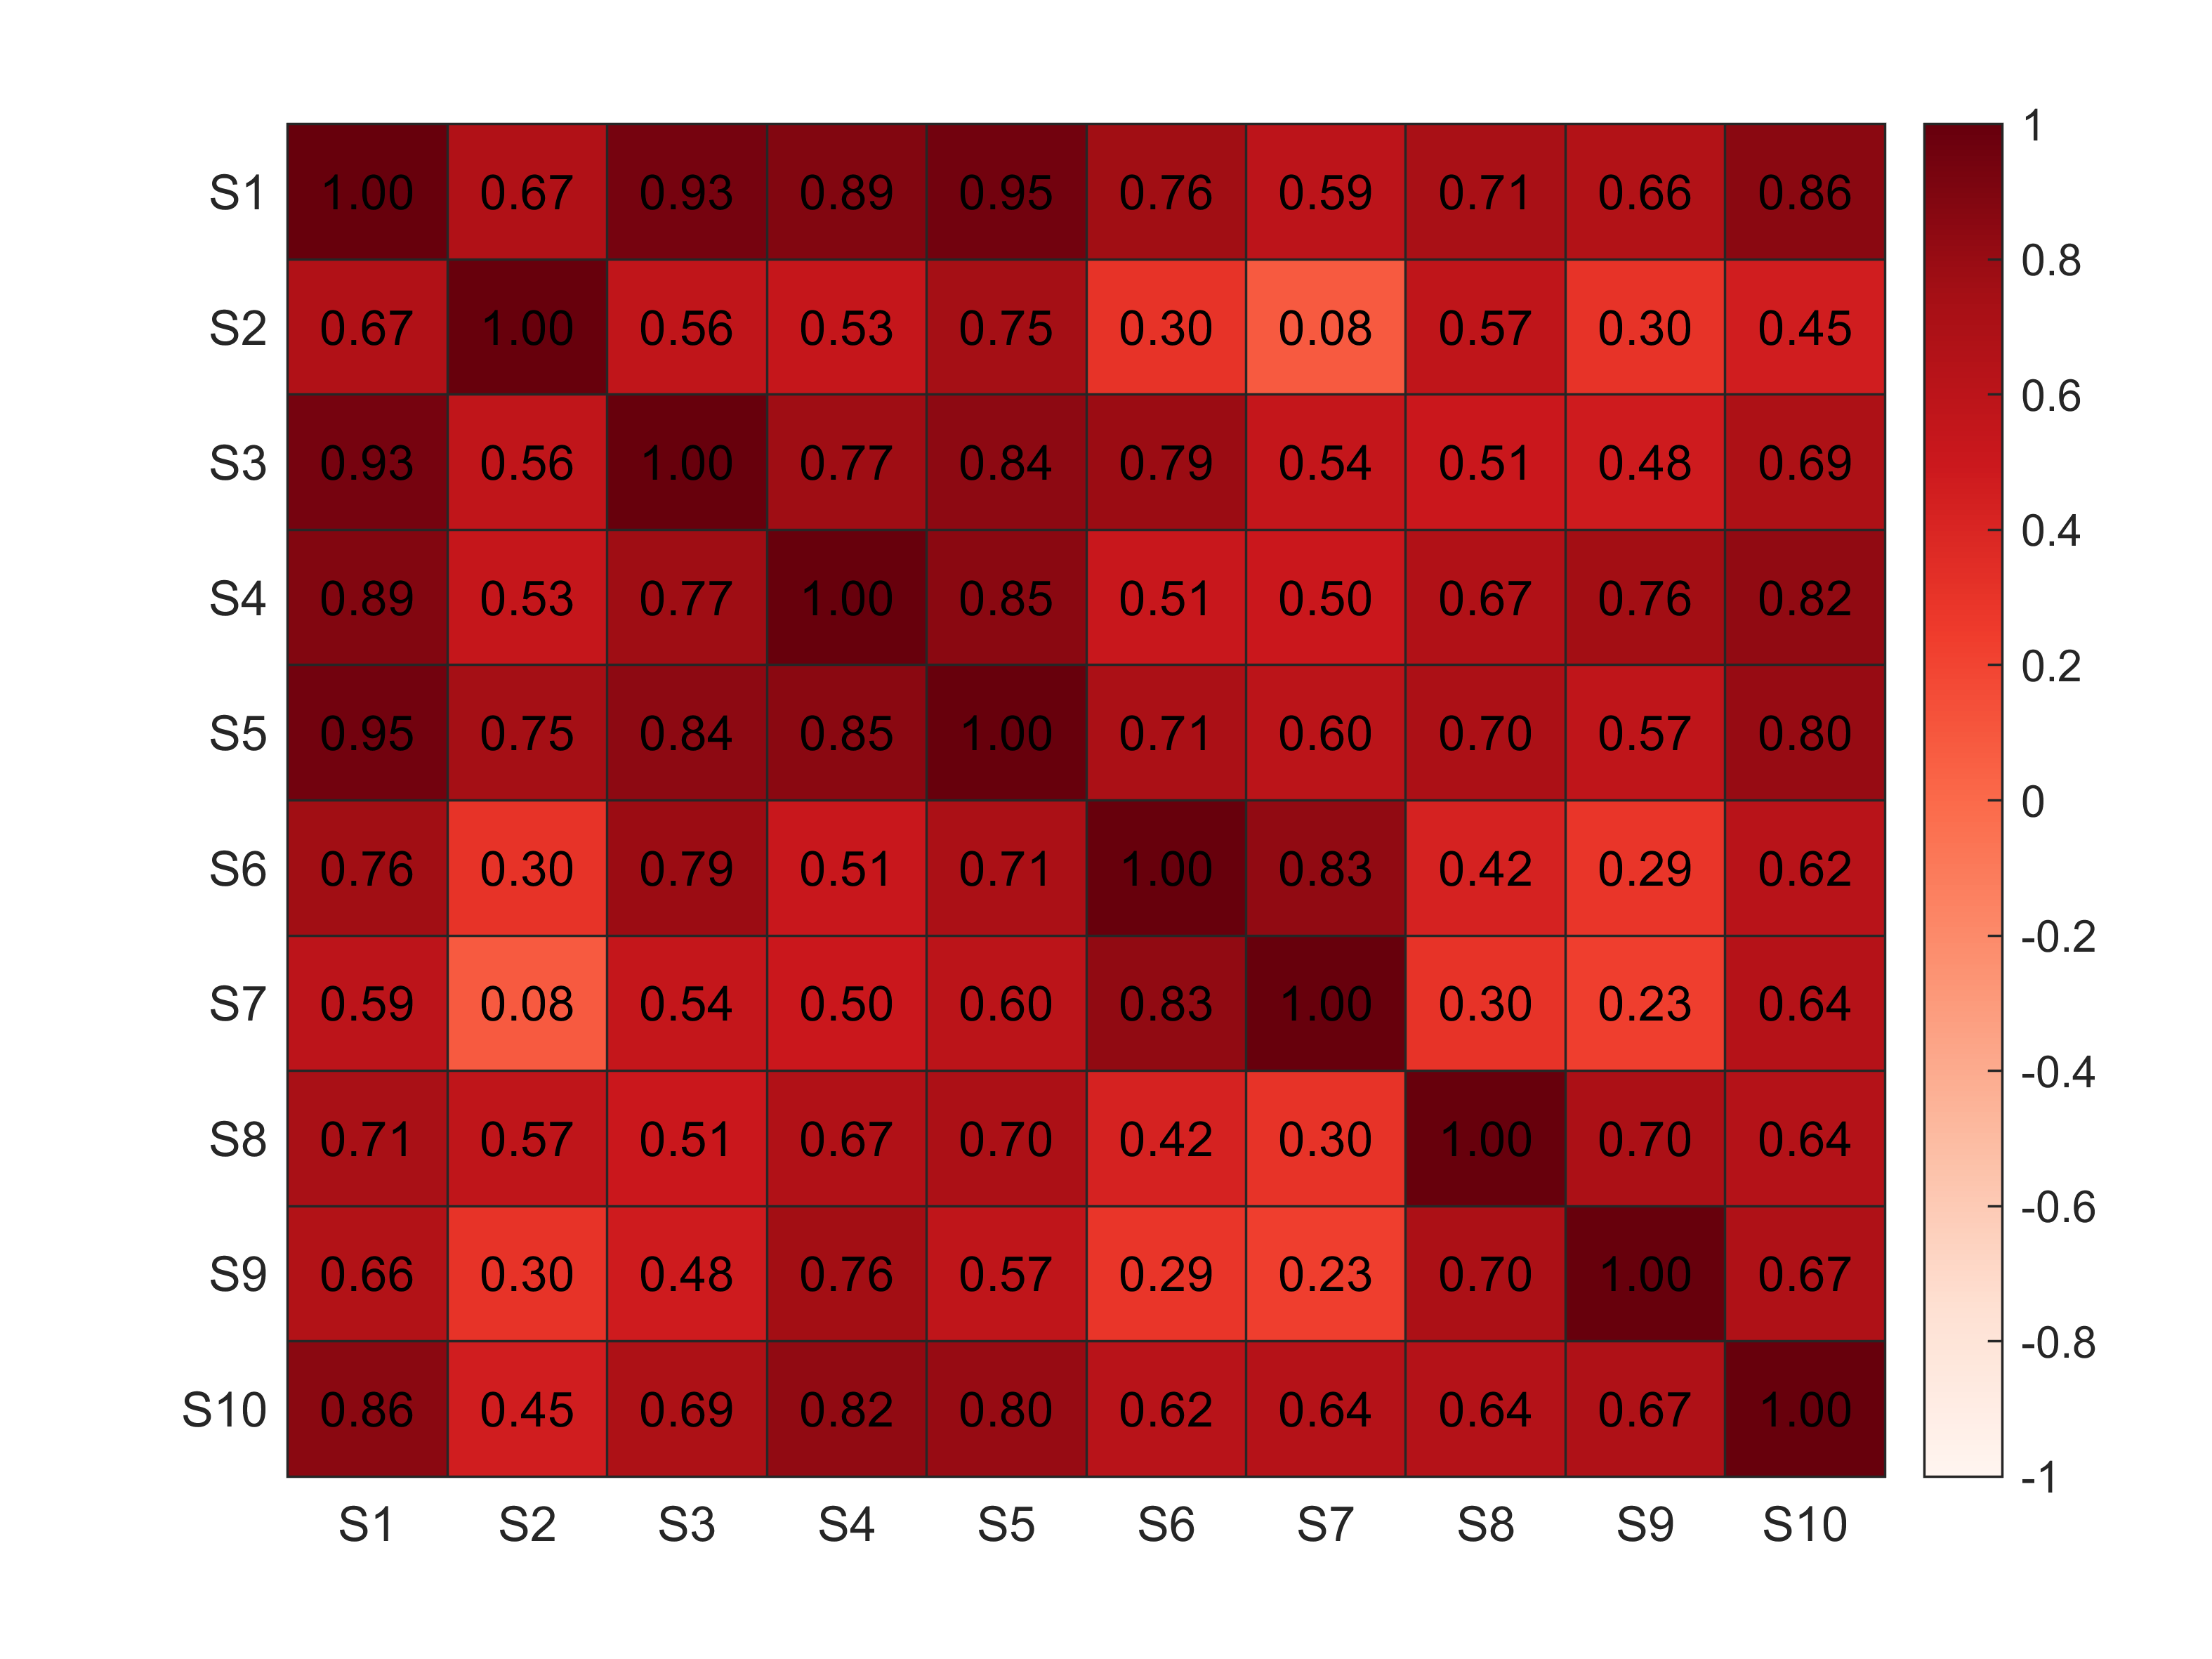
\includegraphics[width=0.48\textwidth]{img/q1_Growth_Rate_Correlation_Matrix20}
			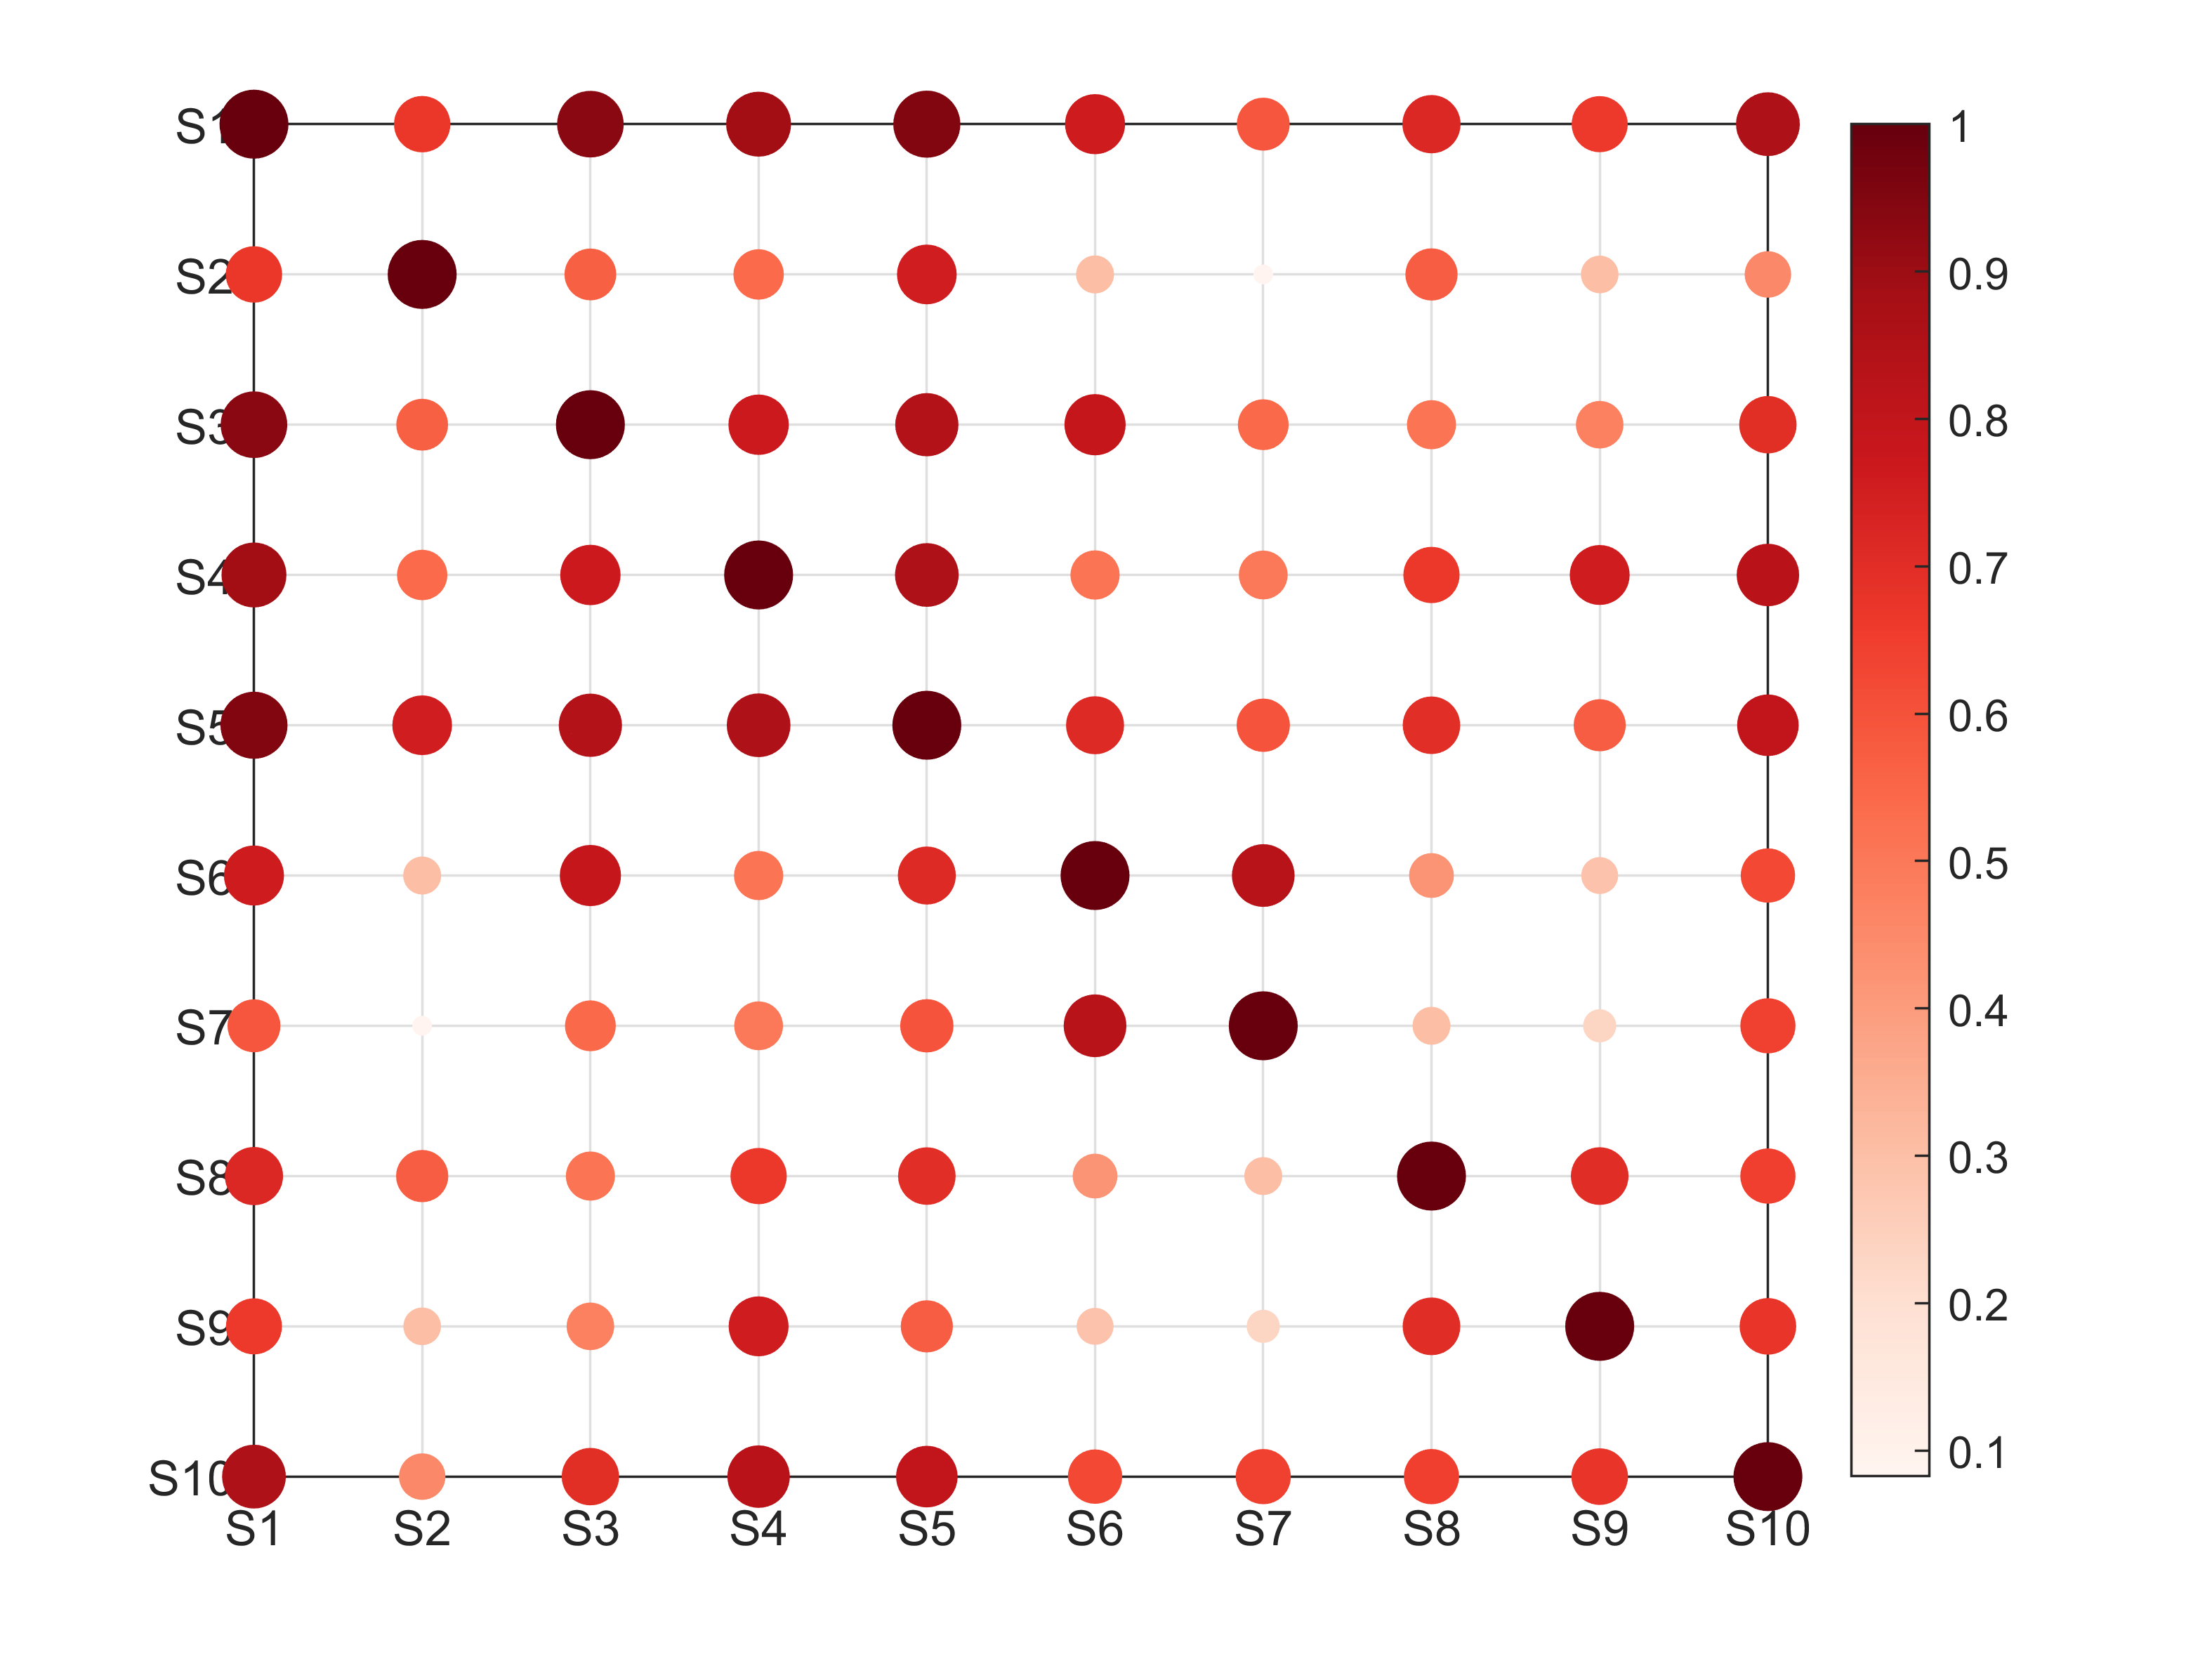
\includegraphics[width=0.48\textwidth]{img/q1_Scatter_Heatmap20} 
		\caption{Pearson correlation coefficient heat distribution.}
		\label{figure4}
	\end{figure}

	In Pearson correlation coefficient, ${(0.8, 1)}$, denotes very strong correlation, ${(0.6, 0.8)}$ denotes strong correlation, ${(0.4, 0.6)}$ denotes medium strength correlation, ${(0.2, 0.4)}$ denotes weak correlation, and ${(0, 0.2)}$ denotes  very weak correlation or no correlation. From the above figure, it can be seen that there is a very strong correlation between wholesale and retail trade and GDP, industry and transportation, storage and postal services. There is a very strong correlation between industry and GDP.
	
	
	
	
%列表
%\begin{enumerate}[\bfseries 1.]
%	\setlength{\parsep}{0ex} %段落间距
%	\setlength{\topsep}{0ex} %列表到上下文的垂直距离
%	\setlength{\itemsep}{0ex} %条目间距
%	\item 
%	\item 
%	\item 
%\end{enumerate}

%AB图
%\begin{figure}[htbp]
 %   \centering    
 %   \subfigure[Data Screening(left)]{				% 图片1([]内为子图标题)						
  %  \includegraphics[width=0.45\textwidth]{Data_Screening(1).png}}			  % 子图1的图片宽度 不能空行
  %  \subfigure[Data Screening(right)]{				% 图片2
  %  \includegraphics[width=0.45\textwidth]{Data_Screening(2).png}}
%	\caption{Data Screening} % 图片标题 
%\end{figure}

\subsection{Establishment and Solution of Linear Programming Models Based on Least Squares Methods}

	The parameters of the linear model were estimated using the least squares method to study the relationship between the amount of investment and the gross product of each industry. The merit of the model fit was assessed by the coefficient of determination $R^2$ to compare the models.

\subsubsection{Preparation of Linear Programming Models Based on Least Squares Methods} 
	Typically, the expression for the form of the linear regression model is:
	
	\begin{equation}
		y = {\beta _0} + {\beta _1}x + \varepsilon
	\end{equation}
	The fitting coefficients are calculated without taking into account the error term $ \varepsilon $, i.e., random errors that cannot be explained by the model.
	

\subsubsection{Establishment of a Linear Programming Model Based on The Least Squares Method}

	The fitting function assumptions for the linear regression for each industry are as follows:
	\begin{equation}
		GD{P_{{S_i}}} = {\beta _i} + {\alpha _i}{X_{{S_i}}}, (i = 2,3,...,10)
	\end{equation}

	where $GDP_{S_i}$ denotes the GDP of the $i$ ($i = 2, 3, \cdots, 10 $) industry, $\alpha_i$, $\beta_i$, ${\delta_i}$ denotes the fit of the $i$ industry, and $X_{S_i}$ denotes the investment amount of the $i$ industry.
	
	$R^2$ denotes the accuracy of the fit, which is expressed as:
	
	\begin{equation}
	{R^{^2}} = 1 - \frac{{\sum\nolimits_{i = 1}^{\rm{n}} {{{({y_i} - {{\hat y}_i})}^2}} }}{{\sum\nolimits_{i = 1}^{\rm{n}} {{{({y_i} - \overline y )}^2}} }}
	\end{equation}

	where $n$ denote the number of industries, $y_i$ denotes the gross production value of the $i$ th industry, ${\hat y_i}$ denotes the forecasted gross production value of the $i$ th industry, and $\overline{y}$ denotes the mean value of the gross production value of the industry. $\sum\nolimits_{i = 1}^{\rm{n}} {{{({y_i} - {{\hat y}_i})}^2}} $ denotes the variance not explained by the model, and $\sum\nolimits_{i = 1}^{\rm{n}} {{{({y_i} - \overline y )}^2}} $ denotes the total variance of the total production value of the industry.
	
	$R^2 = 1$ indicates that all of the variance is explained by the regression model, $0<R^2<1$ indicates that a portion of the variance is explained, and $R^2 = 0$ indicates that the model does not predict better than the prediction using the mean of the industry's total output value.
	
\subsubsection{Solving Linear Programming Models Based on Least Squares Methods}

	Let the number of industries $n=9$, and build different linear regression models for different industries. Construct the design matrix $X$ and estimate the model parameters using least squares, i.e., solve the formal equation:
		\begin{equation}
			({X^T}X)\gamma  = {X^T}y
		\end{equation}
	
	where $\gamma$ is the parameter vector, containing the intercept term and slope, and $y$ is the vector of observations.
	
	Parameter estimation $\hat \gamma$ can be done by:

		\begin{equation}
			\hat \gamma  = {({X^T}X)^{ - 1}}{X^T}y
		\end{equation}

	The slope, intercept and $R^2$ in the linear regression equation for each industry were obtained by solving the above parameters using matlab as follows \ref{sanxianbiao}:
	

\begin{table}[htbp] % 三线表
	\begin{center}
		\caption{Comparison of linear fitting degrees by industry.}
		\label{sanxianbiao}
		\begin{tabular}{c c c c}
			\toprule[2pt]
			\textbf{estate} & \textbf{slope} & \textbf{intercept} & \textbf{$R^2$} \\
			\midrule
			\(S_2\) & 1.67 & 23218.63 & 0.95 \\
			\(S_3\) & 1.04 & 41009.20 & 0.97 \\
			\(S_4\) & -0.19 & 42586.76 & -0.15 \\
			\(S_5\) & 3.56 & 10751.51 & 0.87 \\
			\(S_6\) & 0.59 & 4254.32 & 0.97 \\
			\(S_7\) & 2.11 & 2029.97 & 0.75 \\
			\(S_8\) & 50.78 & 6753.99 & 0.51 \\
			\(S_9\) & 0.41 & -784.52 & 0.98 \\
			\(S_{10}\) & 1.35 & 8516.61 & 0.98 \\
			\bottomrule[2pt]
		\end{tabular}
	\end{center}
\end{table}

	$R^2=1$ When the fit is perfect, ($0.8, 1$) means hte fit is very good, ($0.6, 0.8$) means the fit good, ($0.4, 0.6$) means the fit is fair, ($0.2, 0.4$) means the fit is poor, and ($0, 0.2$) means the fit is very poor.

	The plots of the fitted functions for each industry are shown below:
	
\begin{figure}[H] \centering
	\setlength{\fboxsep}{0pt} % 设置边框间距为0
	\setlength{\fboxrule}{0.5pt} % 设置边框线宽
	
	% 创建一个包含3行3列的表格来摆放图像
	\begin{tabular}{cccc}
		\fbox{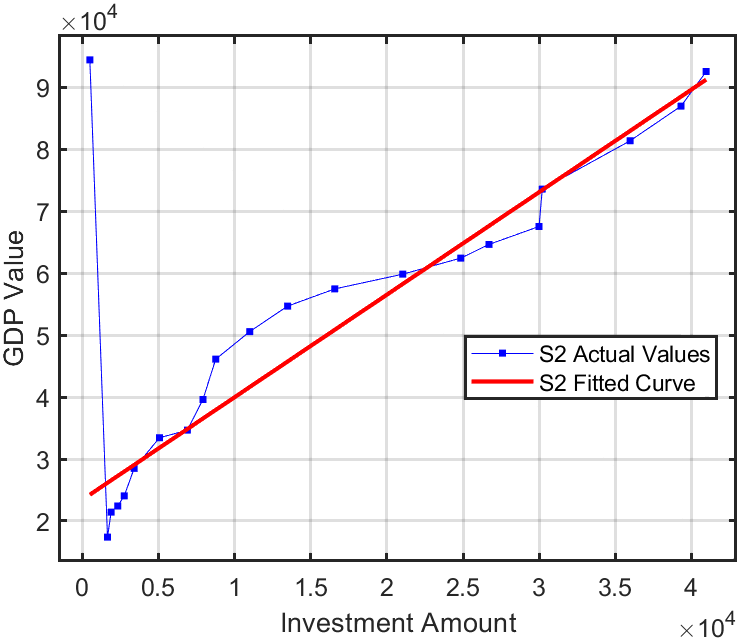
\includegraphics[width=0.288\textwidth]{img/q2_1t_s2}} &
		\fbox{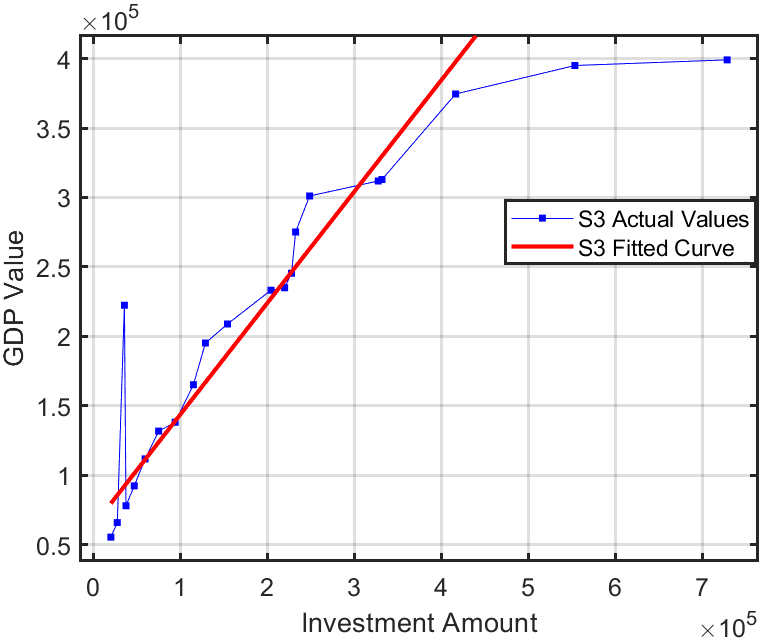
\includegraphics[width=0.288\textwidth]{img/q2_1t_s3}} &
		\fbox{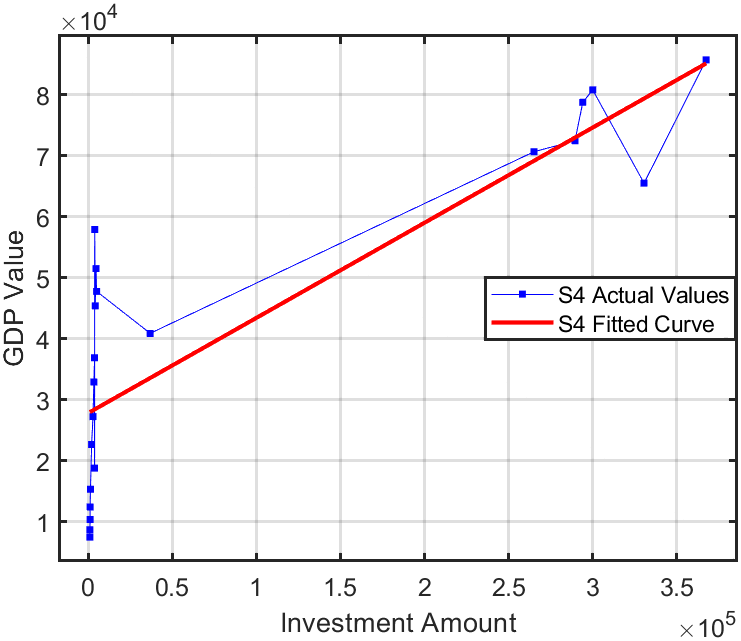
\includegraphics[width=0.288\textwidth]{img/q2_1t_s4}} \\
		
		\fbox{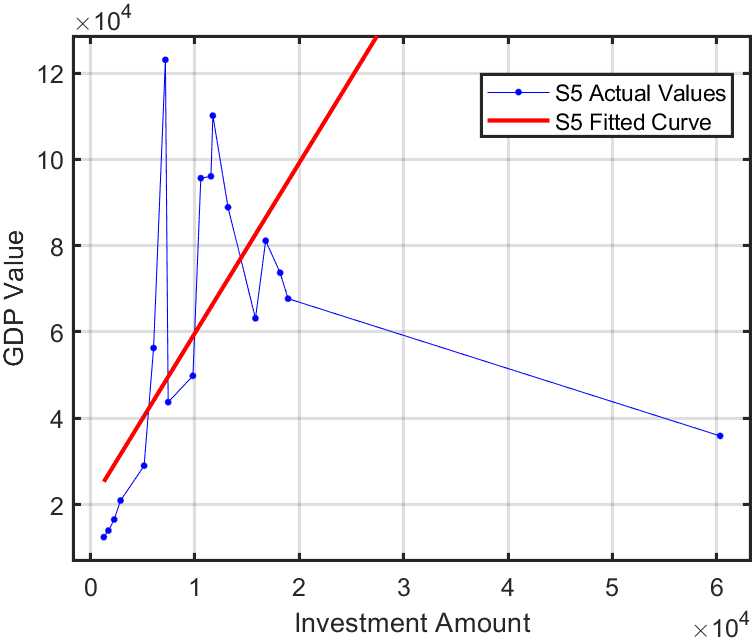
\includegraphics[width=0.288\textwidth]{img/q2_1t_s5}} &
		\fbox{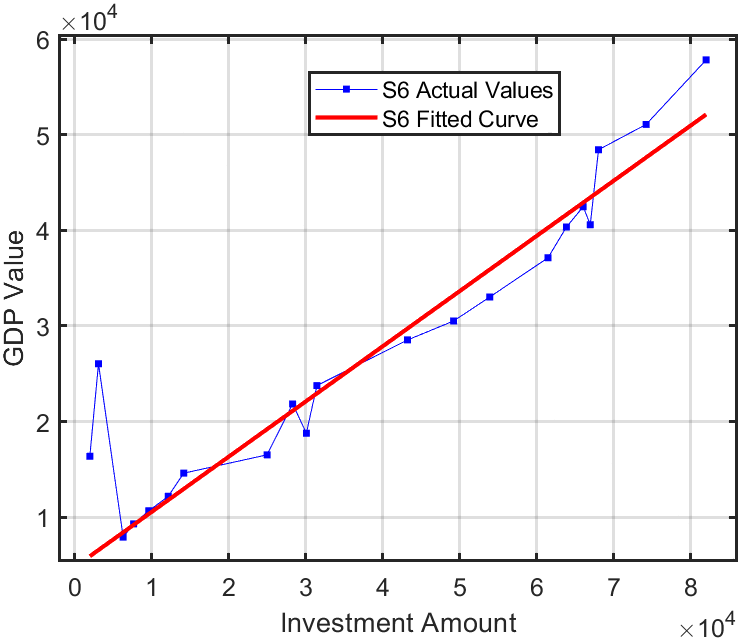
\includegraphics[width=0.288\textwidth]{img/q2_1t_s6}} &
		\fbox{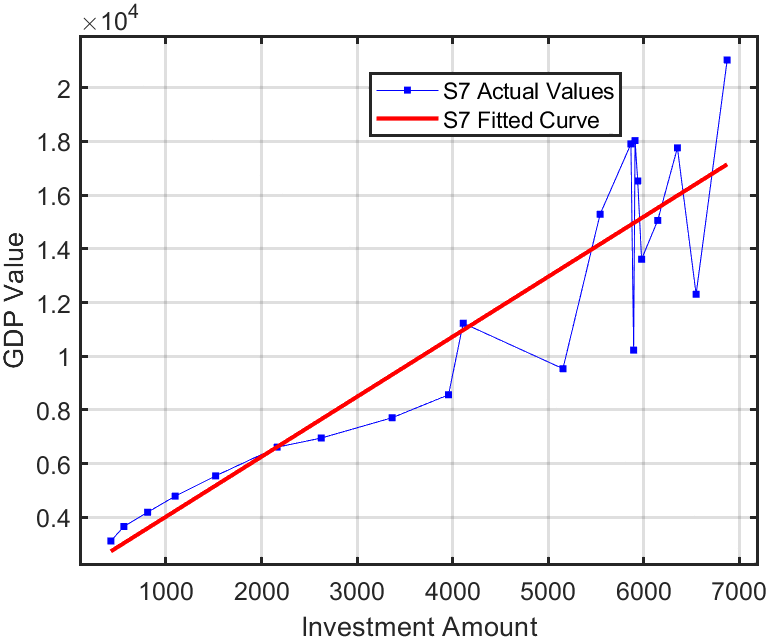
\includegraphics[width=0.288\textwidth]{img/q2_1t_s7}} \\
		
		\fbox{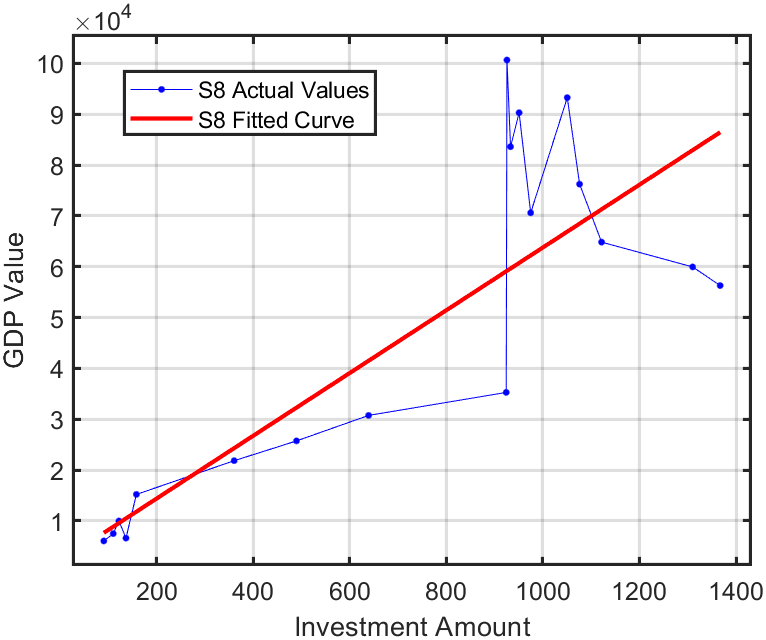
\includegraphics[width=0.288\textwidth]{img/q2_1t_s8}} &
		\fbox{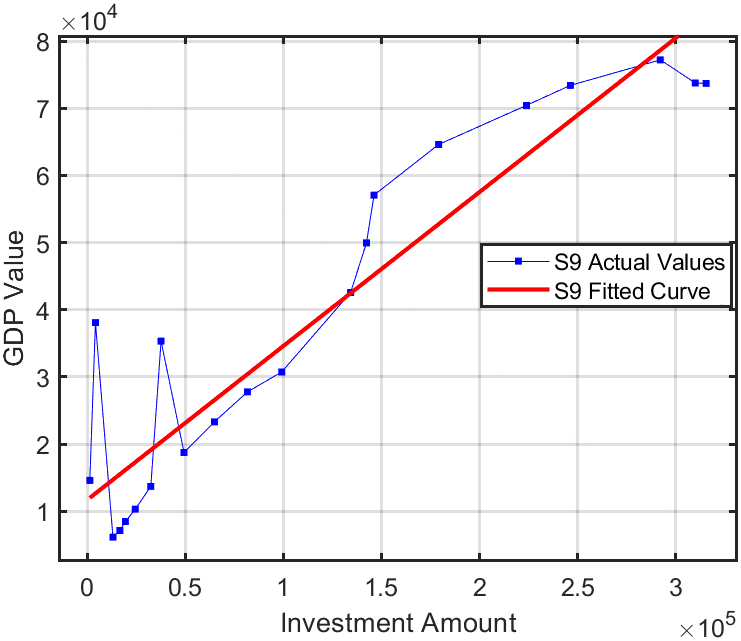
\includegraphics[width=0.288\textwidth]{img/q2_1t_s9}} &
		\fbox{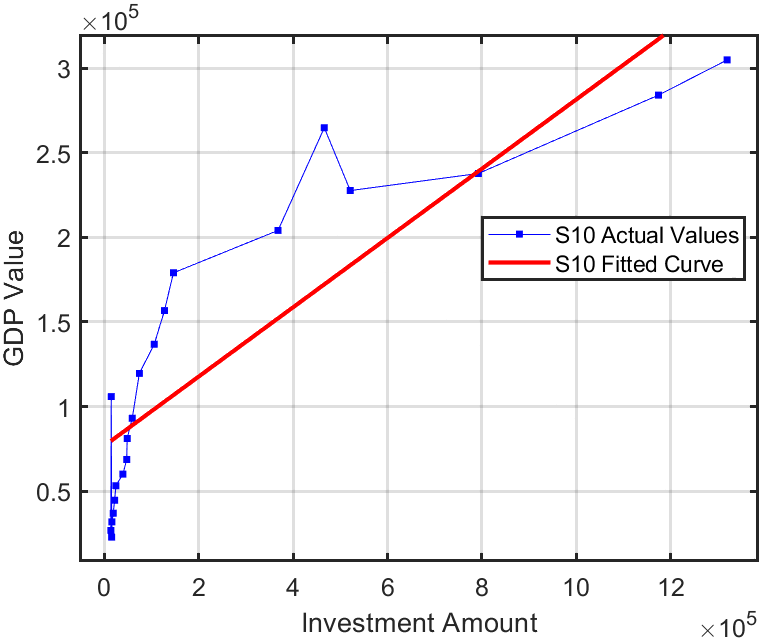
\includegraphics[width=0.288\textwidth]{img/q2_1t_s10}} \\
	\end{tabular}
	
	\caption{Linear fitting functions for nine major industries.} 
	\label{fig:teaser}
\end{figure}

	Combining the images and $R^2$ it is clear that $S_{2}$, $S_{3}$, $S_{5}$, $S_{6}$, $S_{9}$ and $S_{10}$ industry fits very well, but$S_4$ industry has a negative value of $R^2$, which indicates that this industry is not suitable for linear programming. The quadratic polynomial regression model, the exponential regression model, and the logarithmic regression model were built for this industry, and the resulting function plots are as follows Figure\ref{figer3s}.
	
	\begin{figure}[H] \centering
		\setlength{\fboxsep}{0pt} % 设置边框间距为0
		\setlength{\fboxrule}{0.5pt} % 设置边框线宽
		
		% 创建一个包含3行3列的表格来摆放图像
		\begin{tabular}{cccc}
			\fbox{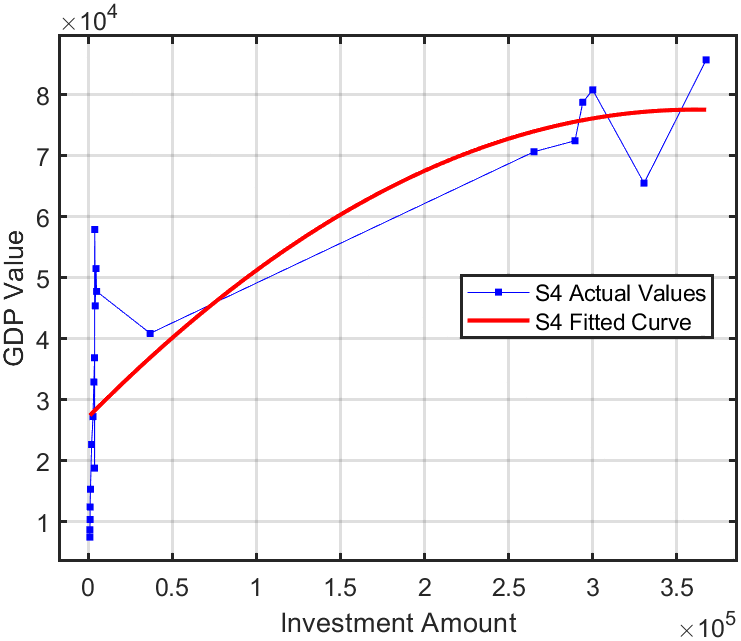
\includegraphics[width=0.288\textwidth]{img/q2_2t_s4}} &
			\fbox{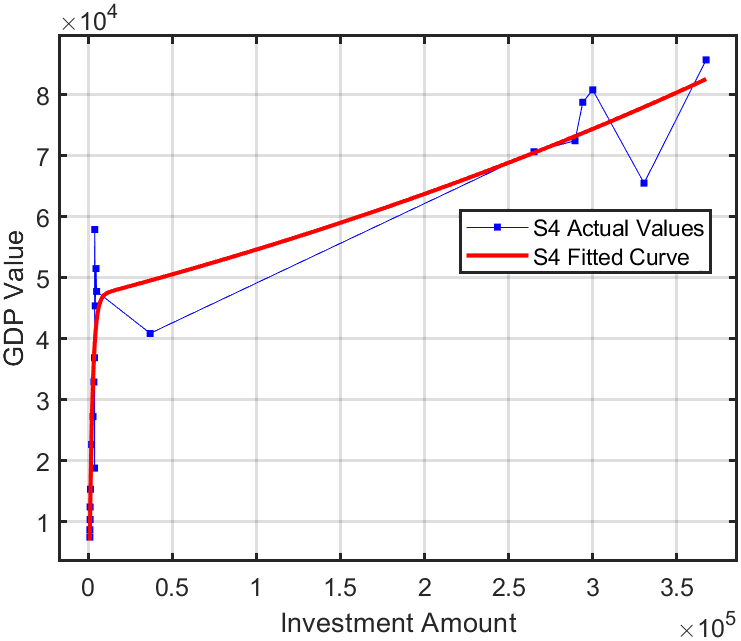
\includegraphics[width=0.288\textwidth]{img/q2_e_s4}} &
			\fbox{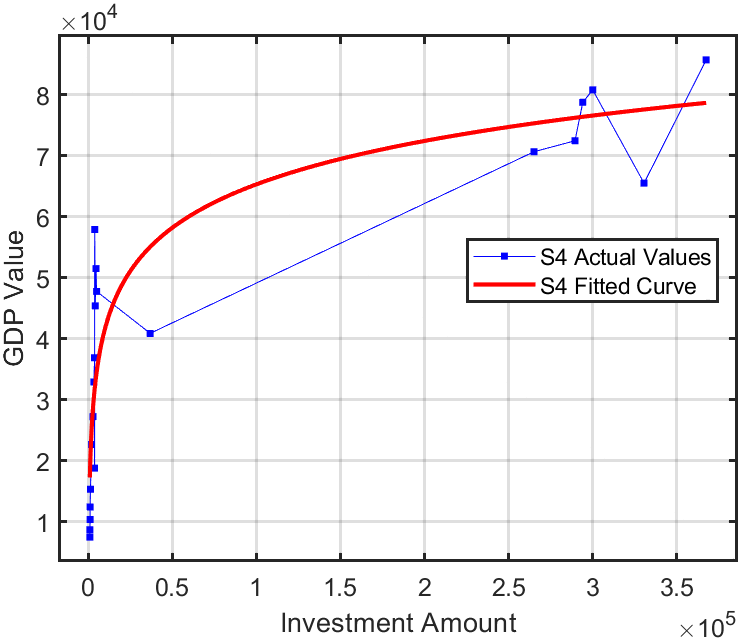
\includegraphics[width=0.288\textwidth]{img/q2_ln_s4}}

		\end{tabular}
		
		\caption{Image of a nonlinear fitting function.} 
		\label{figer3s}
	\end{figure}

	The three regression models corresponding to $R^2$ are shown in the table below Table\ref{tab:regression_comparison}:
	\begin{table}[H]
		\centering
		\caption{Comparison of $R^2$ under different models.}
		\label{tab:regression_comparison}
		\begin{tabular}{lccc}
			\toprule
			& \textbf{quadratic polynomial regression} & \textbf{exponential regression} & \textbf{logistic regression} \\
			\midrule
			$R^2$ & 0.0084 & -0.0043 & 0.0381 \\
			\bottomrule
		\end{tabular}
	\end{table}

	Since there is no significant correlation between the $S_4$ original data for the  industry and there is no significant relationship among the four regression models, the linear regression model is taken as the investment model for the $S_4$ industry in order to simplify the model for this question.

\subsection{Particle Swarm Algorithm Based Linear Programming Model Building and Solving}
	Based on the investment model derived from Problem 2, the optimal solution for investment allocation can be found by particle swarm algorithm.
	
	\subsubsection{ Preparation of a linear programming model based on particle swarm algorithm}
		The steps of the particle swarm algorithm are shown below Figure \ref{figss}.
		
		\begin{figure}[H] % 放置图片的位置
			\centering
			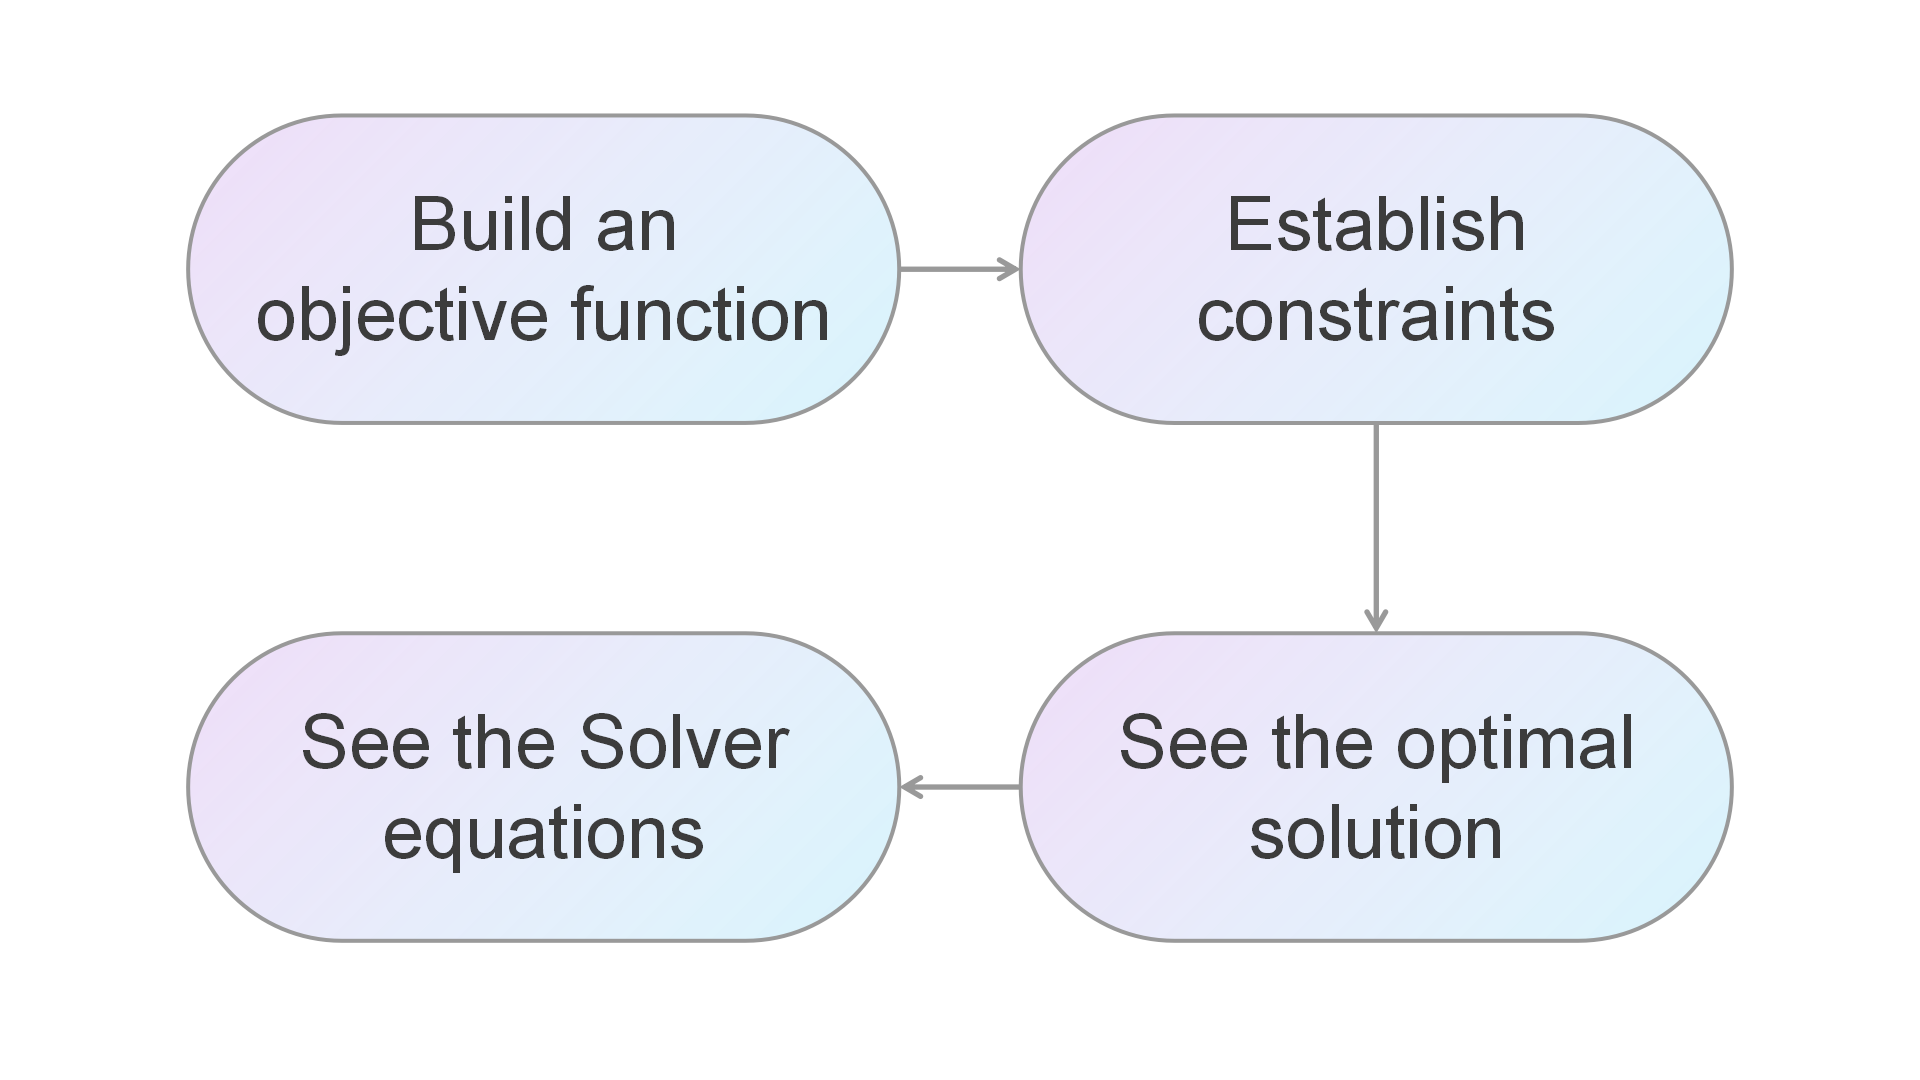
\includegraphics[width=0.8\textwidth]{img/liziqun} % 插入图片,设置宽度为文本宽度的 80%
			\caption{Basic steps of particle swarm algorithm.} % 图片标题
			\label{figss} % 图片标签
		\end{figure}
		
		
	\subsubsection{Modeling of linear programming based on particle swarm algorithm}
		Total GDP is equal to the sum of the GDP of each industry, and profit is GDP minus investment costs:

		\begin{equation}
			profit = GDP - invest
		\end{equation}

	To maximize profit with limited capital, the objective function is:
		\begin{equation}
		\begin{array}{l}
		\max Z = 16715*{I_2} + 10448*{I_3} - 18908*{I_4} + 35585*{I_5} + 5866.8*{I_6}\\
		+ 2111.5*{I_7} + 507.79*{I_8} + 406.9*{I_9} + 1354.3*{I_{10}} + 138337.38
		\end{array}
		\end{equation}
	The constraints are:
	\begin{equation}
		s.t.\begin{aligned}
			& \left\{
			\begin{array}{l}
				I_2 + I_3 + I_4 + I_5 + I_6 + I_7 + I_8 + I_9 + I_{10} \le 1 \\
				I_2 \in (0.073, 1) \\
				I_3 \in (0.309, 1) \\
				I_4 \in (0.054, 1) \\
				I_5 \in (0.075, 1) \\
				I_6 \in (0.04, 1) \\
				I_7 \in (0.015, 1) \\
				I_8 \in (0.04, 1) \\
				I_9 \in (0.044, 1) \\
				I_{10} \in (0.165, 1)
			\end{array}
			\right.
		\end{aligned}
	\end{equation}

	Particle swarm algorithm based on the above conditions leads to an optimal solution. That is, the industry that can realize the maximum profit is obtained and invested in it.

	For investing in three industries to achieve the highest GDP, a linear fit can be made based on the return on investment for each industry to calculate the rate of return for each industry on the next investment. The ROI formula is as follows:
	
	\begin{equation}
	{\alpha _i} = \frac{{{G_i} - {I_i}}}{{{I_i}}}(i = 2,3, \cdot,n)
	\end{equation}

	Based on the projections, the three industries with higher rates of return can be selected and invested in their respective proportions.


\subsubsection{Particle Swarm Algorithm Based Solving of Linear Programming Models}

	The particle swarm algorithm is solved by matlab and the optimal solution is obtained as follows:
	
	\begin{table}[H]
		\centering
		\caption{Investment by industry.}
		\label{tab:solved_values}
		\begin{tabular}{lc}
			\toprule
			\textbf{parameters} & \textbf{Solved value (in  trillion units)} \\
			\midrule
			$Z$ & 13770.82 \\
			$I_2$ & 0.079 \\
			$I_3$ & 0.312 \\
			$I_4$ & 0.054 \\
			$I_5$ & 0.272 \\
			$I_6$ & 0.042 \\
			$I_7$ & 0.016 \\
			$I_8$ & 0.04 \\
			$I_9$ & 0.044 \\
			$I_{10}$ & 0.165 \\
			\bottomrule
		\end{tabular}
	\end{table}

	This shows that GDP can be maximized by investing 0.312 trillion in the $S_3$ industry, 0.272 trillion in the $S_5$ industry, and 0.165 trillion in the $S_{10}$ industry.
	
	\begin{figure}[H] % 放置图片的位置
		\centering
		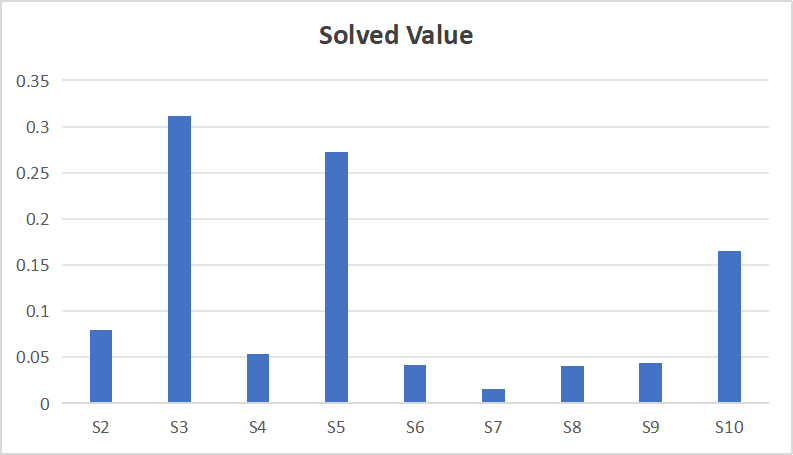
\includegraphics[width=0.8\textwidth]{img/q3} % 插入图片,设置宽度为文本宽度的 80%
		\caption{Proportion of investment allocation.} % 图片标题
		\label{liucheng} % 图片标签
	\end{figure}
	
	From the above figure, it can be seen that $S_3$, $S_5$ and $S_{10}$ industries have the largest solution values. The particle swarm optimization algorithm is performed again for these three industries to solve the best investment ratio as shown in the table below.
	
	
	\begin{table}[H]
		\centering
		\caption{Investment in the three industries.}
		\label{tab:solved_parameters}
		\begin{tabular}{lc}
			\toprule
			\textbf{parameters} & \textbf{Solved value (in trillion units)} \\
			\midrule
			$Z$ & 60279.737 \\
			$X_3$ & 0.309 \\
			$X_5$ & 0.526 \\
			$X_{10}$ & 0.165 \\
			\bottomrule
		\end{tabular}
	\end{table}

\subsection{Modeling and solving for investment elasticity}

	Models are built to calculate and standardize the elasticity values for different industries, to represent the relationship between investment and employment, and to plan investment allocation ratios.

\subsubsection{Preparation of investment elasticity models}

	The cleaned data are first run through an elasticity formula that reflects the impact of investment on employment growth and wage growth \cite{3}. And then the elasticity values are standardized to compare the elasticity values of different industries. The standardized elasticity values obtained in the previous step are further calculated to obtain the composite elasticity values. Finally, the calculation of investment allocation is carried out, in the case of not restricting the number of industries to be invested in, industries with higher comprehensive elasticity will receive more investment; if the investment is restricted to three industries, the three industries with the highest comprehensive elasticity value will be selected and the corresponding investment proportion will be allocated.

\subsubsection{Modeling of investment elasticity}

	The raw data is processed to some extent to become investment growth rate, wage growth rate \cite{5}, and employment growth rate for the next step of analysis.
	The employment elasticity and wage elasticity are calculated for each industry using the following formulas:
		\begin{equation}
			{X_i} = \frac{{{\alpha _i}}}{{{\beta _i}}}
		\end{equation}
	
		\begin{equation}
			{Y_i} = \frac{{{\delta _i}}}{{{\beta _i}}}
		\end{equation}

	$X_i$ denotes the employment elasticity, which reflects the impact of investment on employment growth \cite{3}, $\alpha _i$ denotes the employment growth rate, and $\beta _i$ denotes the investment growth rate. $Y_i$ enotes wage elasticity, which reflects the impact of investment on wage growth, and ${\delta_i}$ denotes wage growth rate. ${i=2, 3, \cdots, 10}$ Indicates industry number.
	
	In order to enable direct comparison of the elasticity values of different industries and to improve the stability of the numerical calculations, the average annual employment elasticity and the flexible wage of each industry are first calculated and finally the following standardized formula is utilized:
	\begin{equation}
		Z = \frac{{(E - \mu )}}{\sigma }
	\end{equation}
			

	$E$ denotes the value of the elasticity, $\mu $ denotes the average annual employment elasticity and flexible wage, and $\sigma $ denotes the difference between the maximum and minimum values of the employment elasticity or flexible wage.
	
	The combined elasticity value is the mean of the sum of the standardized employment elasticity and the standardized wage elasticity. The investment allocation ratio for each industry is calculated from the combined elasticity value using the following formula.

	\begin{equation}
		{N_1} = \frac{T}{{\sum\limits_{i = 1}^n {{T_i}} }}M
	\end{equation}
	The above formula shows the calculation of the sectoral investment allocation ratio	$N_1$ in case there is no restriction on investment in the industry, where $T$ is the value of combined elasticity, $\sum\limits_{i = 1}^n {{T_i}} $ is the value of combined elasticity, and $M$ is the total investment amount.
	
		\begin{equation}
			N_2 = \frac{T'}{\sum_{i=1}^{n} T_i'}
		\end{equation}

	The above formula shows the calculation of industry investment allocation ratio $N_2$ in case of restriction on investment in three industries, where $T$ is the combined elasticity value of the selected industries, $\sum\limits_{i = 1}^n {{T_i}} $ is the combined elasticity value of the selected industries.
	
\subsubsection{Solving the investment elasticity model}

	Using data-processed employment and wage growth rates, the elasticity measures the sensitivity of the amount of investment to the size of the employed population and wages, and calculating the employment elasticity as well as the wage elasticity yields the following Figure \ref{q4_tanxing_work_wage}:
	
		\begin{figure}[H] % 放置图片的位置
		\centering
		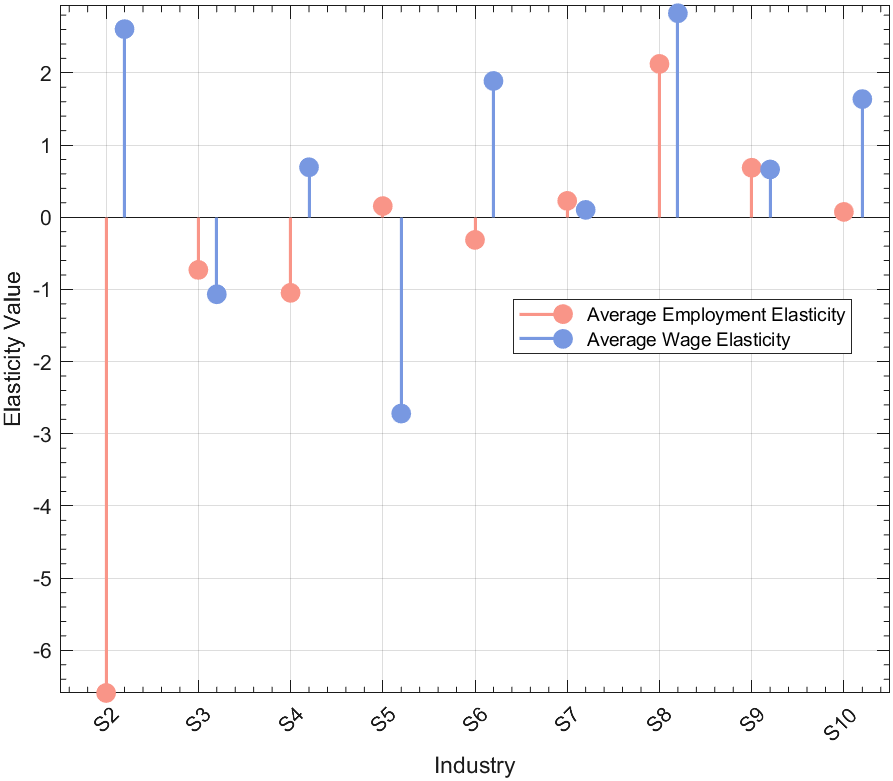
\includegraphics[width=0.8\textwidth]{img/q4_tanxing_work_wage} % 插入图片,设置宽度为文本宽度的 80%
		\caption{Employment elasticity and wage elasticity by industry.} % 图片标题
		\label{q4_tanxing_work_wage} % 图片标签
	\end{figure}

	The impact of investment on employment growth and wage growth can be visualized from the figure above. For industry $S_1$, the employment fell while wages rose; employment and its wages fell in $S_3$ industries. Therefore, both should be considered when planning investment programs.
	
	The combined elasticity is obtained through employment and wage elasticity, which is then calculated to obtain the investment allocation ratio, as shown below:
	
	\begin{figure}[H]
		\centering
		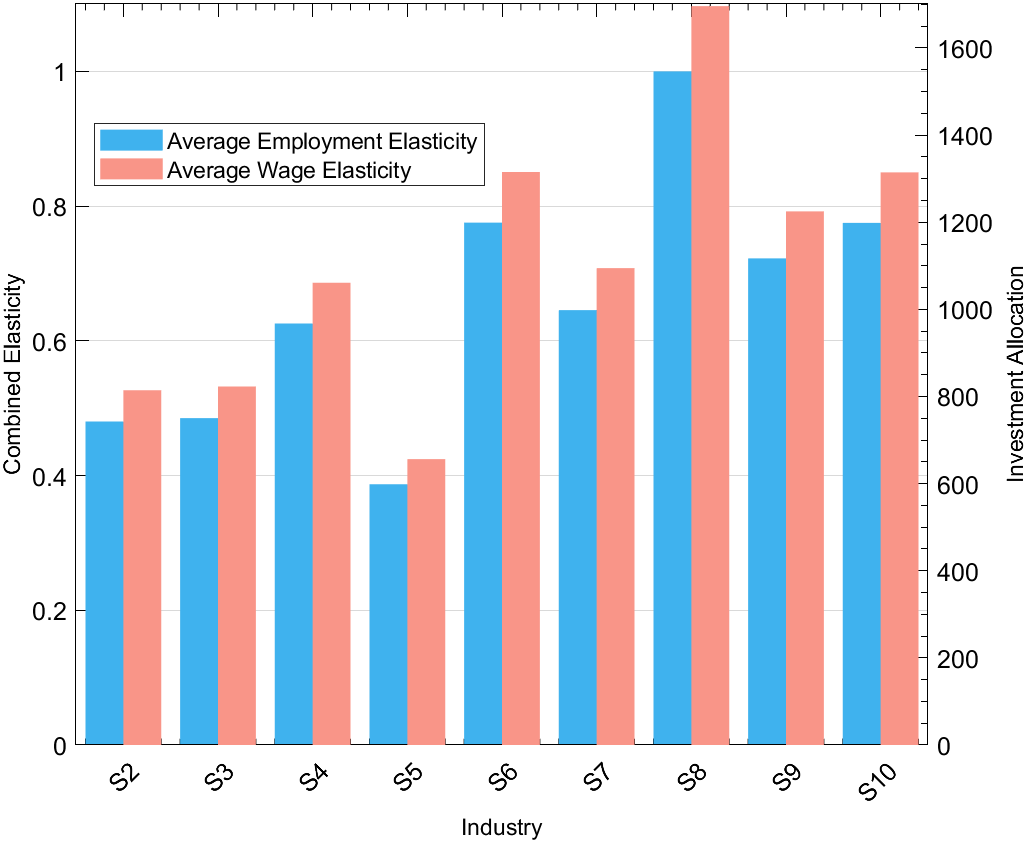
\includegraphics[width=0.48\textwidth]{img/q4_all_tanxing_invest}
		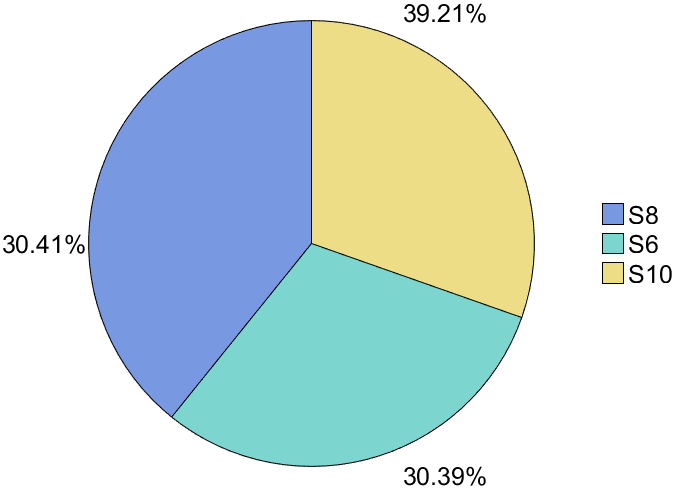
\includegraphics[width=0.48\textwidth]{img/q4_three_best} 
		\caption{Investment allocation.}
		\label{threess}
	\end{figure}
	
	
	The left panel shows a graph of the composite elasticity indicator, with the blue bars showing the employment elasticity and the red bars showing the wage elasticity, the left vertical coordinate showing the result of the calculation based on these two variables, and the right vertical coordinate showing the amount of investment to be allocated.
	The chart on the right shows the proportion of investment that should be allocated to achieve the highest GDP if investment is limited to three sectors.
	
\subsection{Multi-Objective Planning Modeling and Solving}
	A multi-objective planning model is used to weight the independent variables using hierarchical analysis, and the optimal solution is found by particle swarm algorithm.
	
	\subsubsection{Preparation of multi-objective planning models}
	In multi-objective optimization problems, there are often conflicting situations between different objective functions. Through the assignment, the relative importance of each objective can be clarified, so as to find a reasonable balance point between these multiple conflicting objectives.
	
	The hierarchical analysis method (AHP) is utilized to assign weights to the objective functions in order to avoid conflicts between the objective functions as shown in the figure below:
	
	\begin{figure}[H] % 放置图片的位置
		\centering
		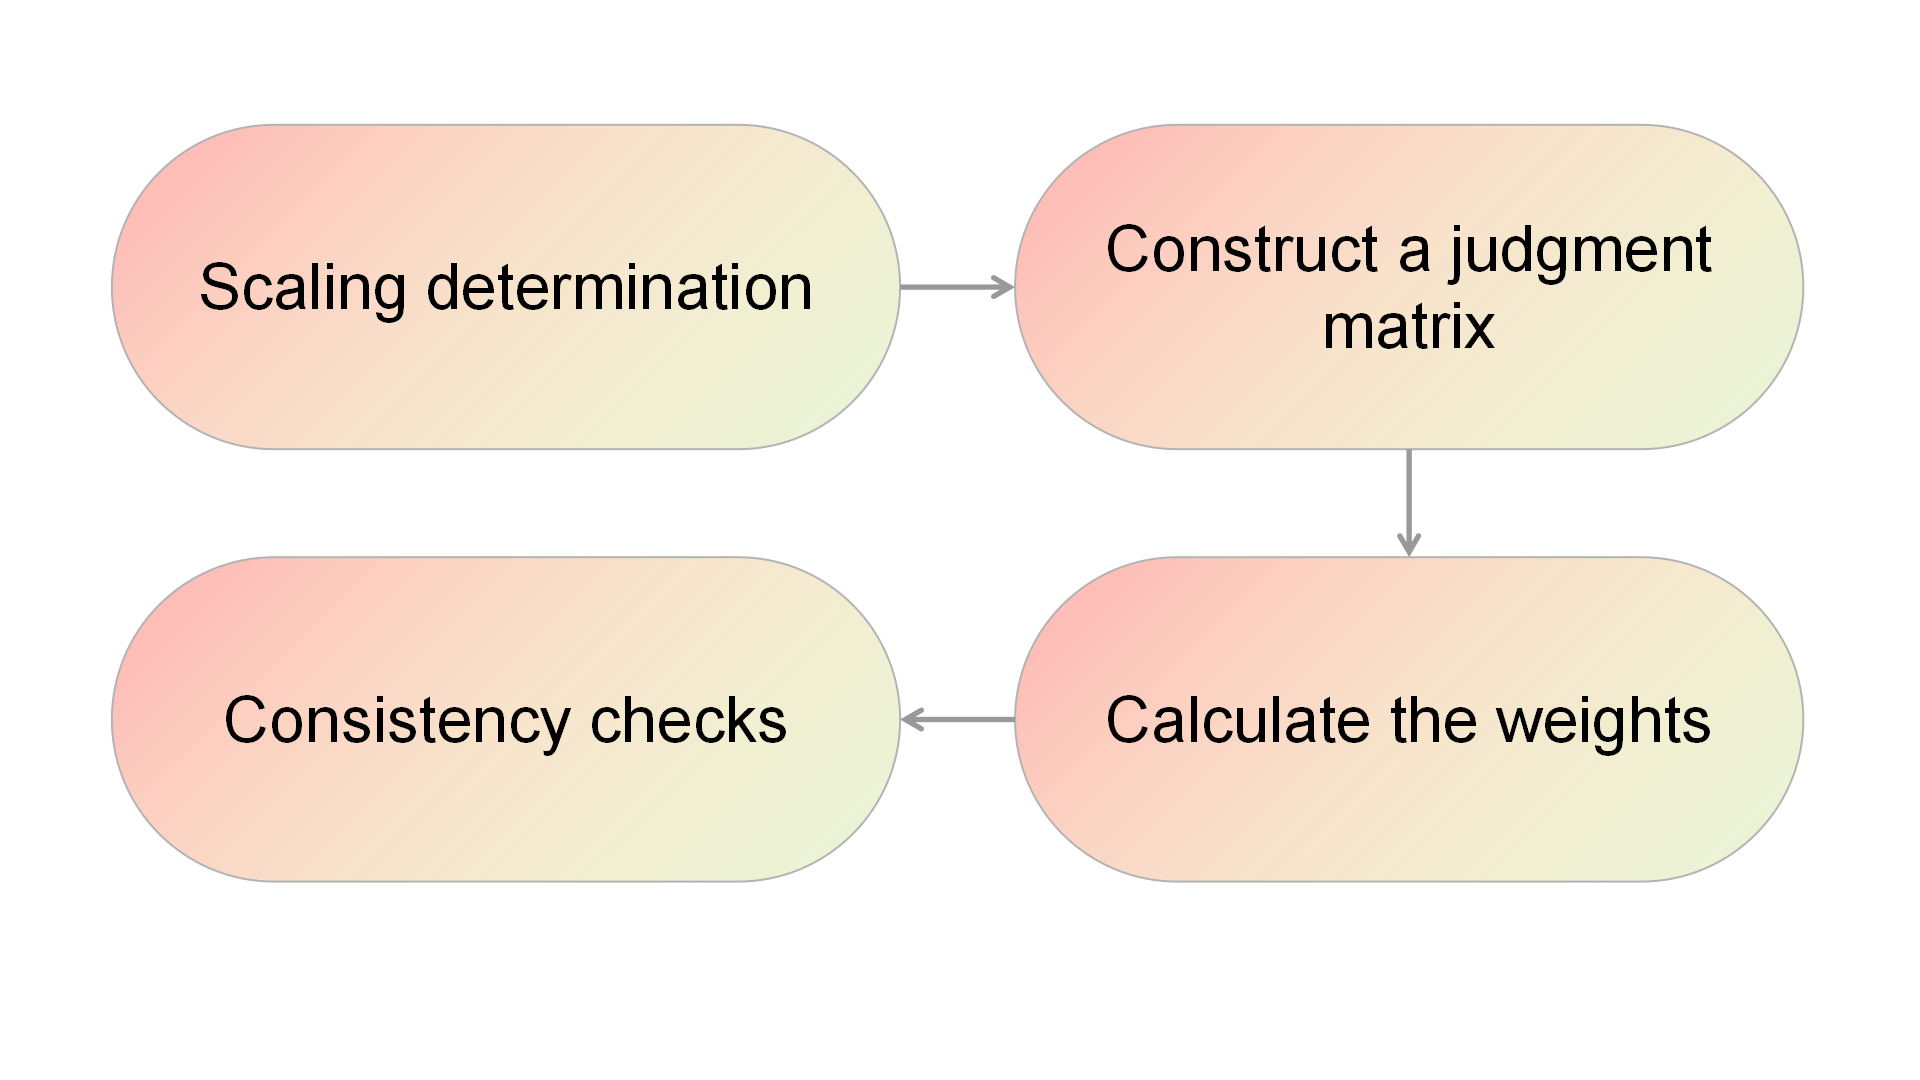
\includegraphics[width=0.8\textwidth]{img/AHP} % 插入图片,设置宽度为文本宽度的 80%
		\caption{The basic steps of analytic hierarchy process.} % 图片标题
		\label{AHP} % 图片标签
	\end{figure}
	
	
	The weight values can be calculated by sum and product method. Subsequently, these weight values are substituted into the objective function and finally the optimal investment allocation scheme is calculated with the help of Particle Swarm Optimization (PSO) algorithm.
	
	\subsubsection{Multi-objective planning modeling}
	
	A multi-objective planning model is a mathematical model used to optimize multiple objectives simultaneously. In order to increase employment while achieving the highest total GDP, a multi-objective planning model can be used to optimize employment as well as GDP at the same time; however, there is often a conflict between these objectives.
	
	Define the objective function.
		\begin{equation}
			\max Y = nF + \left( {1 - n} \right)G
		\end{equation}
	
	Clarify constraints:
		\begin{equation}
			s.t.\left\{ \begin{array}{l}
				F =  - 5.4 \times {10^{ - 7}}{I_2} - 5.9 \times {10^3}{I_3} + 9.9 \times {10^{ - 6}}{I_4}\\
				+ 1.7 \times {10^{ - 7}}{I_5} - 1.3 \times {10^{ - 8}}{I_6} + 1.3 \times {10^{ - 6}} \cdot {I_7} - 3 \times {10^{ - 5}}{I_8} + 1.6 \times {10^{ - 7}}{I_9} + 1.4 \times {10^{ - 6}}{I_{10}} + 0.9\\
				G = 16715{I_2} + 10448{I_3} - 18908{I_4} + 35585{I_5}\\
				+ 5866.8{I_6} + 2111.5{I_7} + 507.8{I_8} + 406.9{I_9} + 1354.3{I_{10}} + 138337.3\\
				{I_2} + {I_3} + {I_4} + {I_5} + {I_6} + {I_7} + {I_8} + {I_9} + {I_{10}} \le 1\\
				{I_2} \in (0.073,1)\\
				{I_3} \in (0.309,1)\\
				{I_4} \in (0.054,1)\\
				{I_5} \in (0.075,1)\\
				{I_6} \in (0.04,1)\\
				{I_7} \in (0.015,1)\\
				{I_8} \in (0.04,1)\\
				{I_9} \in (0.044,1)\\
				{I_{10}} \in (0.165,1)
			\end{array} \right.
		\end{equation}
	
	Assigning weights to conflicting objectives through hierarchical analysis to determine the relative importance of each objective. The judgment matrix is processed using normalization in the sum-product method and the weight vector is calculated.
	
	The computed weights are substituted into the objective function to transform the multi-objective optimization problem into a single-objective optimization problem.
	
	Finally the particle swarm optimization algorithm is used to solve the single objective optimization problem to find the optimal solution.
	
	\subsubsection{Multi-objective planning model solution}
	
	The weight of $F$ is obtained by hierarchical analysis as $\frac{1}{3}$ and and the weight of $G$ is $\frac{2}{3}$.
	
	The particle swarm algorithm is solved and the optimal solution obtained is as follows:
	
	 
	 \begin{table}[H]
	 	\centering
	 	\caption{Investment in various industries.}
	 	\label{resultss}
	 	\begin{tabular}{lc}
	 		\toprule
	 		\textbf{Parameter} & \textbf{Solved Value} \\
	 		\midrule
	 		Objective Value (z) & 31859.477 \\
	 		$X_2$ & 0.096 \\
	 		$X_3$ & 0.326 \\
	 		$X_4$ & 0.054 \\
	 		$X_5$ & 0.098 \\
	 		$X_6$ & 0.064 \\
	 		$X_7$ & 0.039 \\
	 		$X_8$ & 0.064 \\
	 		$X_9$ & 0.068 \\
	 		$X_{10}$ & 0.186 \\
	 		\bottomrule
	 	\end{tabular}
	 \end{table}
	 
	 From the Table \ref{resultss}, it is clear that the solution values of $S_3$, $S_5$, $S_{10}$ are the best solution values.
	 
	 	\begin{figure}[H] % 放置图片的位置
	 	\centering
	 	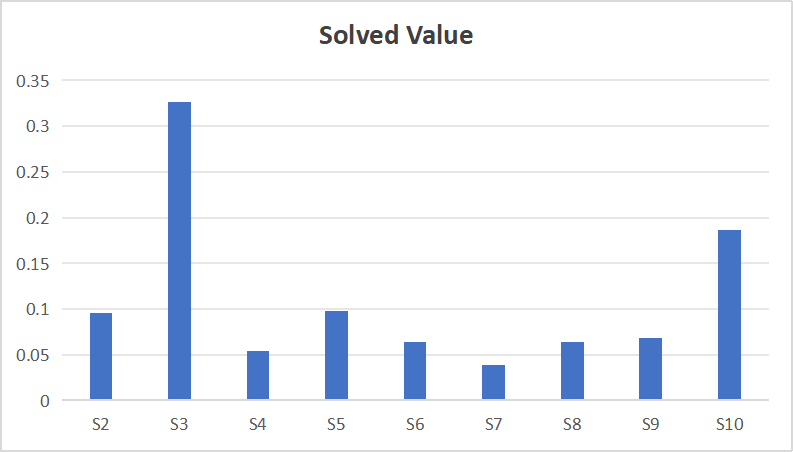
\includegraphics[width=0.8\textwidth]{img/q5} % 插入图片,设置宽度为文本宽度的 80%
	 	\caption{Proportion of investment allocation.} % 图片标题
	 	\label{q5} % 图片标签
	 \end{figure}
 
	 From the above figure, it can be seen that $S_3$, $S_5$ and $S_{10}$ industries have the largest solution value. Next, the particle swarm optimization algorithm is performed again for these three industries to solve for the optimal investment ratio.
	 
	 
\section{Evaluation and generalization of the model}
\subsection{Advantages of the model}
	\begin{itemize}  %无序列表
		\item Based on the model of Pearson's correlation coefficient, the interrelationship between industries is discussed from two aspects. The consideration is more comprehensive, which makes the results more convincing.
		\item The multi-objective planning model takes into account the conflict problem brought about by multiple optimization objectives, uses the hierarchical analysis method to weight the optimization objectives, and finally uses the particle swarm algorithm to derive the optimal solution, which uses a variety of analytical methods, is more rigorous in its consideration, and the results are more accurate.
	\end{itemize}

\subsection{Disadvantages of the model}
	\begin{itemize}  %无序列表
		\item The simplification of the real economic environment by the investment resilience model may result in a model that does not fully capture the complexity of emergency activities and that relies heavily on the quality and reliability of the data.
		\item Least squares-based models are sensitive to outliers and cannot deal directly with categorical variables, with limited predictive power.
	\end{itemize}

	 
	 
	 
	 
	 
	 
	 
	 
	


% 参考文献,此处以 MLA 引用格式为例
\clearpage   %另起一页继续写。这时,你最好使用“\clearpage” 
\begin{thebibliography}{99}
	
	\bibitem{1} % 格兰杰因果检验文献
	Diks, Cees, and Valentyn Panchenko. "A new statistic and practical guidelines for nonparametric Granger causality testing." Journal of Economic Dynamics and Control 30.9-10 (2006): 1647-1669.

	\bibitem{2} % 皮尔逊相关系数文献
	Cohen, Israel, et al. "Pearson correlation coefficient." Noise reduction in speech processing (2009): 1-4.
	
	\bibitem{3} % 经济增长的就业弹性2000-2017
	Morén V, Wändal E. The employment elasticity of economic growth-A global study of trends and determinants for the years 2000-2017[J]. 2019.

	
	\bibitem{4} % GDP-就业弹性
	Burgi C, Hovhannisyan S, Mondragon-Velez C. GDP-Employment Elasticities across Develo** Economies[R]. The World Bank, 2024.

	
	\bibitem{5} % 劳动力需求弹性与最低工资
	Danziger L. The elasticity of labor demand and the minimum wage[J]. Journal of Population Economics, 2009, 22: 757-772.
	
	

	
	

	
\end{thebibliography}


%% 下面不知道是个啥,先注释掉了
% \includepdf[pages={1,2}]{Memo.pdf} 

%\newpage
%\begin{center}
%	\Huge{\texorpdfstring{%
%			Memorandum}{Memorandum}}
%	\addcontentsline{toc}{section}{Memorandum} % Add entry to the table of contents
%\end{center}

%\leaders\vrule width \linewidth\vskip 2pt % Add a bold horizontal line with a specified line width
%\vspace{-10pt} % Adjust the vertical space

%\begin{flushleft}
%	\textbf{To:} xx \\
%	\textbf{From:} Team XX \\
%	\textbf{Date:} January 22nd, 2024 \\
%	\textbf{Subject:} Your Subject Here% 主题
%\end{flushleft}

%\vspace{-10pt} % Adjust the vertical space
%% 上面不知道是个啥,先注释掉了

\leaders\vrule width \linewidth\vskip 2pt % Add a thin horizontal line with the same width


	
\newpage
\appendix
%\section{Appendix:1}

%\lstinputlisting[language=python]{code/code1.py}%引用代码文件
%报错别担心,是因为代码内部索引出了问题

%\section{Appendix:2}












   
   


\end{document}  % 结束